\documentclass[english,brazil]{iftex}

% ------------------------------------------------------------------------
% Pacotes
% ------------------------------------------------------------------------
% Pacote para destaque de códigos fonte
\usepackage{fancyvrb}

% Pacote para símbulos extras
\usepackage{textcomp}

% Pacote para tabelas
\usepackage{tabularx}

\usepackage{caption}

% Algoritmos
\usepackage[noend]{algpseudocode}
% Comandos para traduzir as instruções do pacote de algoritmos
\algrenewcommand\algorithmicrequire{\textbf{Entrada:}}
\algrenewcommand\algorithmicensure{\textbf{Condição:}}
\algrenewcommand\algorithmicend{\textbf{fim}}
\algrenewcommand\algorithmicif{\textbf{se}}
\algrenewcommand\algorithmicthen{\textbf{então}}
\algrenewcommand\algorithmicelse{\textbf{senão}}
\algrenewcommand\algorithmicfor{\textbf{para}}
\algrenewcommand\algorithmicforall{\textbf{para todo}}
\algrenewcommand\algorithmicdo{\textbf{faça}}
\algrenewcommand\algorithmicwhile{\textbf{enquanto}}
\algrenewcommand\algorithmicrepeat{\textbf{repita}}
\algrenewcommand\algorithmicuntil{\textbf{até que}}
\renewcommand{\Return}{\State \textbf{retorne} }

% Comando simples para exibir comandos Latex no texto
\newcommand{\comando}[1]{\textbf{$\backslash$#1}}
\newcommand{\ifmgtex}[1]{IFMG\TeX}

% Estilo de capítulo
% \chapterstyle{bianchi}


% ------------------------------------------------------------------------
% Configurações do Documento
% ------------------------------------------------------------------------
\titulo{Comparação do Desempenho Multi-Core de Arquiteturas RISC e CISC: Um Estudo de Caso Entre Computador Desktop e o Raspberry Pi}
\autor{Paulinelly de Sousa Oliveira}
\local{Bambuí - MG}
\data{15}{Dezembro}{2017}

% Instituição
\instituicao{Instituto Federal de Educação, Ciência e Tecnologia de Minas Gerais}
\unidade{\textit{campus} Bambuí}
% Os possíveis tipos de trabalhos são: monografia, dissertacao ou tese
\tipotrabalho{monografia}
\curso{Bacharel}{Engenharia de Computação}

\areaconcentracao{Computação de Alto Desempenho}
% Orientação
\orientador{Prof. Dr. Laerte Mateus Rodrigues}
\coorientador[Coorientador]{Prof. Carlos Renato Nolli}
% Caso o coorientador seja de outra instituição
%\coorientadorinstituicao{Instituição da Coorientadora}

% Membros da banca examinadora (além do orientador e coorientador)
\membrobanca{Prof. Me. Ciniro Aparecido Leite Nametala}{Instituto Federal de Minas Gerais - \textit{campus} Bambuí}
\membrobanca{Prof. Me. Francisco Heider Willy dos Santos}{Instituto Federal de Minas Gerais - \textit{campus} Bambuí}

% ------------------------------------------------------------------------
% Ficha catalográfica (Obrigatória)
% ------------------------------------------------------------------------
% Caso o comando \fichacatalografica seja definido, a ficha catalográfica
% será inserida no verso da folha de rosto.
% Entre em contato com a biblioteca para obter a ficha catalográfica em
% arquivo PDF. Essa ficha só será inserida no documento após a sua defesa.
\inserirfichacatalografica{ficha_catalografica}

% ------------------------------------------------------------------------
% Folha de aprovação (Obrigatória)
% ------------------------------------------------------------------------
% O comando \inserirfolhaaprovacao{} gera a folha de aprovação para ser
% assinada. Após a defesa esta folha deve ser digitalizada em um arquivo
% PDF e inserida pelo comando \inserirfolhaaprovacao{arquivo}
\inserirfolhaaprovacao{folhaprovacao}

% Dedicatória (Opcional)
\inserirdedicatoria{
A Deus, pela força para lutar e chegar até aqui.	

Aos meus pais, à minha irmã e meus amigos, pelo incentivo e motivação para alcançar meus sonhos.

A todos que contribuíram e/ou torceram por mim.
}

% Agradecimentos (Opcional)
\inseriragradecimentos{
Agradeço a Deus por te concedido a mim esta grande oportunidade e dado forças em todos os momentos difíceis. Agradeço aos meus pais (José Vicente e Vera Lúcia) e a minha irmã (Patrícia) por terem acreditado em mim e por todo o apoio, confiança e por abraçarem este sonho comigo. Agradeço meu orientador (Laerte), co-orientador (Renato Nolli) e aos demais professores pela ajuda, paciência, conselhos e por todo conhecimento que me passaram, permitindo que eu chegasse aqui. Agradeço aos meus amigos, colegas de sala e curso que me ajudaram direta ou indiretamente. A todos que de alguma forma contribuíram: meu muito obrigado!!
}

% Epígrafe (Opcional)
\inserirepigrafe{
    ``A imaginação é mais importante que a ciência, porque a ciência é limitada, ao passo que a imaginação abrange o mundo inteiro.''\\
    (Albert Einstein)
        
         
    ``Por mais que a ciência evolua e que a tecnologia avance jamais ela vai decifrar a mente humana, pois cada cabeça é um mundo e cada ser humano uma história, jamais caberá numa tese ou num fundamento. Isso faz da humanidade e seu imaginário imensamente complexos e hierárquicos.''\\
    (Afonso Allan)
}

\resumo{
	Os sistemas embarcados estão cada vez mais presentes em nosso cotidiano. Modelos como a Raspberry, Orange Pi, Beaglebone, dentre outros vêm se tornando cada vez mais populares, principalmente em aplicações domésticas e/ou de baixo custo. Este trabalho apresenta um comparativo de desempenho entre um computador \textit{desktop} e uma placa Raspberry Pi modelo 3B. A fim de avaliar os diferentes tipos de processamento, foi utilizado para a análise um algoritmo genético, uma vez que seu código possui baixa granularidade, aplicado na resolução do problema do Caixeiro Viajante. Foram testadas entradas de 5, 10, 15 até 100 cidades, tanto de forma sequencial quanto de forma paralela na placa e no computador, com a finalidade de verificar o desempenho de cada arquitetura de acordo com o tamanho da entrada. Uma amostra, de 50 execuções, com entrada fixa de 30 cidades, também foi realizada em cada uma das arquiteturas (sequencial e paralelo) a fim de verificar aspectos como comportamento ao longo do tempo, entre outros. Os resultados mostram que o desempenho da Raspberry Pi é inferior ao do computador. Este já era um resultado esperado visto que se trata de uma arquitetura embarcada que possui recursos limitados, além de recursos como memória primária e secundária mais lenta que a de um computador. Entretanto, a placa apresentou melhor eficiência na utilização de seus núcleos em relação ao computador. Conclui-se portanto, que a Raspberry Pi é uma alternativa barata e eficiente para sistemas de baixo custo ou que não tenham tempo de resposta como fator crítico.
}
\palavraschave{Raspberry Pi. Desempenho. Paralelo. Sequencial.}


% ------------------------------------------------------------------------
% Keywords e abstract
% ------------------------------------------------------------------------
\abstract{
Embedded systems are increasingly present in our daily lives. Models such as raspberry, orange Pi, Beaglebone, among others have become increasingly popular, especially in domestic and / or low-cost applications. This work presents a performance comparison between a desktop computer and a Raspberry Pi model 3B card. In order to evaluate the different types of processing, a genetic algorithm was used for its analysis, since its code has low granularity, applied in the problem solving of the Traveling Salesman. Five, 10, 15 to 100 cities entries were tested, both sequentially and in parallel on the board and without a computer, in order to verify the performance of each architecture according to the size of the entrance. A sample, of 50 runs, with fixed input of 30 cities, was also performed in each of the series architectures (sequential and parallel) in order to verify how behavior over time, among others. The results show that the performance of raspberry Pi is lower than that of the computer. This was the same expected as an expected problem, but there are memory resources as well as features such as primary and secondary memory that are slower than a computer. However, a board had better use of its cores in relation to the computer. For example, a Raspberry Pi is an inexpensive and efficient alternative for low-cost systems and has no response time as a critical factor.
}
\keywords{Raspberry Pi. Performance. Parallel. Sequential.}
                % Resumo e Abstract (Obrigatórios)
\inserirlistafiguras                     % Lista de Figuras (Opcional)
%\inserirlistaquadros                     % Lista de Quadros (Opcional)
%\inserirlistatabelas                     % Lista de Tabelas (Opcional)
%\inserirlistaalgoritmos                  % Lista de Algoritmos (Opcional)
\inserirlistacodigos                     % Lista de Códigos (Opcional)
%\inserirlistasiglas{\begin{itemize}[]
\item[ABNT] - Associação Brasileira de Normas Técnicas
\item[IFMG] - Instituto Federal de Educação, Ciência e Tecnologia de Minas Gerais
\item[SQL] - \textit{Structured Query Language}
\item[TCC] - Trabalho de conclusão de curso
\end{itemize}
}      % Lista de Siglas (Opcional)
%\inserirlistasimbolos{\begin{itemize}[]
  \item $\mathbb{X}$ -- Variável X
  \item $\mathsf{I\!R}$ -- Conjunto dos números reais
\end{itemize}
}  % Lista de Símbolos (Opcional)

\begin{document}

% -----------------------------------------------------------------------------
% Gera elementos pré-textuais
% -----------------------------------------------------------------------------
\maketitle

% -----------------------------------------------------------------------------
% Capítulo: Introdução
% -----------------------------------------------------------------------------
\chapter{Introdução} \label{cap:introducao}

Atualmente, existe uma necessidade de computadores para processamento com grande carga de trabalho, devido a novas demandas que vêm surgindo nas mais diversas atividades e áreas do conhecimento - principalmente com simulações de problemas relacionados à ciência e à engenharia. Nesse contexto, o conjunto de dados a ser tratado torna-se cada vez maior devido à facilidade de seu armazenamento. \cite[p.~16]{lima:2016:implantacao}. 

Ao longo dos anos, várias técnicas foram utilizadas para melhorar a organização do computador a fim de aumentar a velocidade de processamento, como por exemplo, o uso de memória virtual, unidades de armazenamento externas que não usam discos, hierarquia de barramentos, redução do tamanho dos componentes do microprocessador (o que reduz a distância entre os componentes), \textit{pipelines}\footnote{É uma técnica de implementação de processadores que permite a sobreposição temporal das diversas fases de execução das instruções, aumentando a taxa de instruções iniciadas e terminadas por unidade de tempo. O \textit{pipeline} não reduz o tempo gasto para completar cada instrução individualmente. \cite{stallings:2002:arquitetura}.} etc. Na arquitetura também houve melhorias, como previsão de desvio, análise do fluxo de dados, execução especulativa, dentre outros. \cite{stallings:2002:arquitetura}. Ainda assim, o equilíbrio do desempenho foi necessário para evitar que as melhorias de um componente fossem anuladas pelos atrasos de outros, das quais podem-se citar:    

\begin{enumerate}
	\item Desenvolvimento da hierarquia de memória (consiste em múltiplos níveis de memória com diferentes velocidades e tamanhos);
	\item memória \textit{cache};
	\item caminhos de dados entre memória e processador mais largos;
	\item chips de memória mais inteligentes porque o desenvolvimento da memória principal não acompanhou o do processador.
\end{enumerate}

O projeto do conjunto de instruções implementado em cada arquitetura é fator fundamental para um bom desempenho de acordo com as aplicações do sistema computacional, em que as principais abordagens são a RISC (\textit{Reduced Instruction Set Computer}\footnote{\textbf{Português}: Computador com um conjunto reduzido de instruções.}) e a CISC (\textit{Complex Instruction Set Computer}\footnote{\textbf{Português}: Computador com um conjunto complexo de instruções.}). A RISC possui filosofia de um conjunto de instruções pequeno, simples e de tamanho fixo, que resulta na simplicidade, rapidez e baixo custo da Unidade de Controle (UC). Por outro lado, a CISC possui instruções complexas (arquitetura complexa) que simplificam e facilitam a construção de compiladores, o que faz a compilação de programas complexos gerar menos instruções de máquina (menos acessos a memória para buscar instruções deixa a arquitetura mais rápida).

Contudo, mesmo com estes recursos, ainda existem limites físicos, como a frequência suportada pelo silício. \cite{stallings:2002:arquitetura}. Desta forma, para contornar o problema os projetistas de processadores começaram a colocar vários núcleos num mesmo chip a fim de ser possível o processamento paralelo real.

\begin{citacao}
	Para resolver esses problemas, os designers de processadores passaram a projetar circuitos que pudessem processar dados em paralelo, ou seja, ao invés de tentarem aumentar o poder de processamento de um único núcleo do processador, incluindo mais transistores, os designers passaram a considerar a criação de processadores com muitos núcleos em um único circuito integrado. Tais circuitos são conhecidos como processadores \textit{multicore}. Ao tirar proveito do paralelismo com processadores compostos por vários núcleos, foi possível elevar o poder de processamento a taxas mais altas do que as que vinham sendo alcançadas quando apenas um núcleo era utilizado. \cite{lima:2016:implantacao}.
\end{citacao}

Desde os trabalhos de \citet{vonnewmann:1945:first}, arquiteturas paralelas já eram consideradas soluções com maior capacidade de processamento em execuções com grandes volumes de processamento. Nos anos 70, quando as tecnologias computacionais passaram a não ser mais suficientes para suprir as demandas de processamento, deu-se início à utilização de técnicas de concorrência\footnote{Designa situações nas quais diferentes processos competem pela utilização de algum recurso (processador, memória, dispositivos periféricos etc) ou	cooperam para a realização de uma mesma tarefa. A concorrência pode ser física (múltiplos	processadores independentes) ou lógica (divisão	do tempo de	um	processador	- \textit{time-sharing}). \cite{silberschatz:2008:sistemas}}. para se ter maior desempenho. Limitações, como altos custos, tendenciaram o desenvolvimento de sistemas com vários núcleos juntos, nos chips de microprocessadores, processadores e até mesmo dos supercomputadores. Assim, tem-se várias unidades ativas (ou núcleos) trabalhando de forma paralela na mesma aplicação para que se tenha uma redução no tempo de execução da mesma. \cite{navaux:2011:fund_arquiteturas}.

%\textbf{Fonte:} <http://homepages.dcc.ufmg.br/~rimsa/documents/decom009/lessons/Aula09.pdf>.

Mesmo com avanços consideráveis na arquitetura e na organização de computadores, ao nível de software também foram desenvolvidas técnicas para se obter melhores resultados na resolução de problemas, isso porque existem alguns problemas que não podem ser solucionados com melhorias no hardware, conforme citado anteriormente. Essas técnicas nem sempre garantem o melhor resultado, mas garantem uma boa solução para o problema. Os algoritmos bio-inspirados (que são uma sub-classe da Computação Natural) têm grande importância nesse cenário por serem utilizados em vários tipos de problemas, como reconhecimento de padrões e otimização, por exemplo. A Figura \ref{figura:int_001} mostra divisões e subdivisões da computação natural enquanto a Figura \ref{figura:int_002} mostra os principais algoritmos dentro da sub-classe algoritmos bio-inspirados. \cite{rossi:2009:ajuste}.

\begin{figure}[htb]  
	\centering
	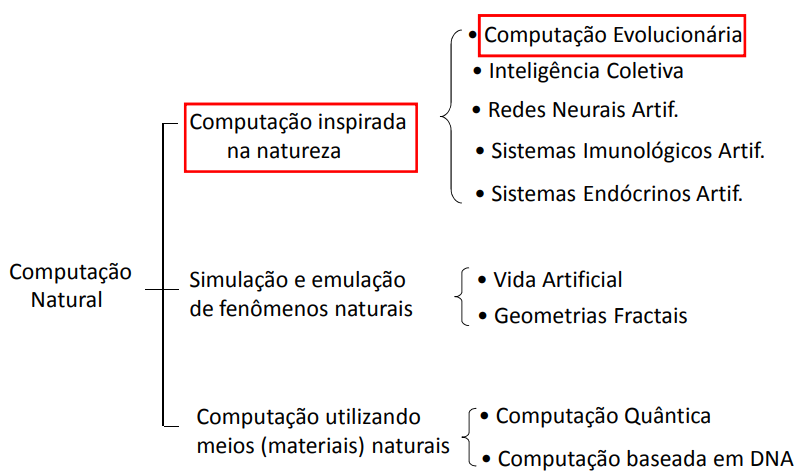
\includegraphics[width=.8\textwidth]{figuras/int_001}
	\caption[Computação Natural]{A Computação Natural possui três subdivisões, sendo elas computação inspirada na natureza ou algoritmos bio-inspirados (computação evolucionária, inteligência coletiva, redes neurais artificiais, sistemas imunológicos artificiais e sistemas endócrinos artificiais), simulação e emulação de fenômenos naturais (vida artificial e geometriais fractais) e a computação utilizando meios físicos naturais (computação quântica e computação baseada em DNA).}
	\ Fonte: \cite{pappa:2015:conceitos}. 
	\label{figura:int_001}
\end{figure}

\begin{figure}[htb]  
	\centering
	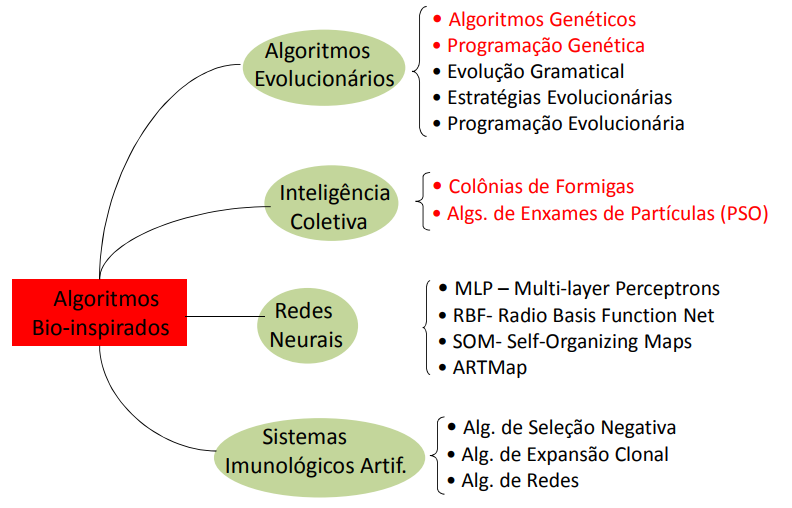
\includegraphics[width=.8\textwidth]{figuras/int_002}
	\caption[Algoritmos bio-inspirados]{Algoritmos bio-inspirados são divididos em: algoritmos evolucionários, inteligência coletiva, redes neurais e sistemas imunológicos artificiais.}
	\ Fonte: \cite{pappa:2015:conceitos}. 
	\label{figura:int_002}
\end{figure}

Além desses avanços, \citet{fuller:2011:computing} mostram que em função do ciclo virtuoso em que a tecnologia se encontra, a aplicação da computação em diversos outros sistemas podem ser vistos, como por exemplo, nos atuais \textit{smartphones}, smarTV's e sistemas embarcados que possuem componentes para computação de propósito geral e específico. Um destes modelos é o Raspberry Pi (basicamente é um pequeno computador) que possui processador, memória, comunicação com dispositivos de entrada e saída, entre outros.

Sendo assim, este trabalho apresenta o desenvolvimento de uma metodologia de comparação do desempenho de programas de forma sequencial e também de forma paralela em duas diferentes arquiteturas, ambas de propósito geral: plataforma Raspberry Pi e um computador \textit{desktop}. Vale ressaltar que o objetivo não é testar qual arquitetura é melhor em relação a outra, mas sim quão bom pode ser o desempenho de uma arquitetura embarcada se comparada ao de um computador comum.

\section{Objetivo Geral}
\label{subsecao:objetivo_geral}

Comparar o desempenho computacional paralelo e sequencial do Raspberry Pi em relação à computadores \textit{desktops}.

\subsection{Objetivos Específicos}
\label{subsecao:objetivos_especificos}

\begin{enumerate}
\item Definir o algoritmo a ser utilizado no trabalho a fim de utilizar o máximo possível do hardware em ambos os cenários.

\item Adaptar ou implementar o algoritmo para execução utilizando programação paralela.

\item Avaliar o desempenho computacional nas 2 arquiteturas propostas.
\end{enumerate}

\section{Justificativa}
\label{secao:justificativa}

Inicialmente, justifica-se esta pesquisa por demonstrar o uso de um computador de baixo custo que apresenta desempenho significativo e que está se tornando cada vez mais popular nos dias atuais, em comparação com um computador que já é utilizado. Outra justificativa é a carência de estudos comparativos de desempenho entre sistemas RISC e CISC. Além disso, fez-se a utilização de uma técnica que foi desenvolvida como solução para melhorar o desempenho dos processadores, que é a programação paralela, aproveitando todos os núcleos disponíveis. Como foi apresentado anteriormente, processadores \textit{multicore} são uma das soluções desenvolvidas para melhorar a capacidade de processamento visto que já não está sendo possível diminuir o tamanho físico dos transistores com a atual tecnologia de semicondutores. 

Assim, ressalta-se que em nossa instituição não há trabalhos científicos utilizando o Raspberry Pi, sendo assim este trabalho serve de alicerce para futuros trabalhos.

\section{Organização do Trabalho}
\label{secao:organizacao_trabalho}

Para um melhor entendimento desta monografia, o mesma foi dividida em capítulos. O capítulo 2 apresenta o referencial teórico, em que são descritos todos os termos e elementos necessários para uma melhor compreensão desta obra. O capítulo 3 apresenta a revisão de literatura, em que é mostrado o que existe de correlato, quais foram suas metodologias e resultados e, ao final como este trabalho se difere dos demais. O capítulo 4 apresenta os materiais e métodos utilizados para o desenvolvimento. Em outras palavras são descritas as técnicas e métricas utilizadas nesta produção. O capítulo 5 apresenta os resultados e discussões obtidos após a execução da metodologia descrita no capítulo 4 e faz uma comparação com os resultados da literatura descritos no capítulo 3. O capítulo 6 apresenta as conclusões obtidas com base nos resultados descritos no capítulo 5 e nos objetivos proposto no capítulo 1, quais limitações foram notadas, quais possíveis trabalhos futuros podem desenvolvidos. Por fim, o capítulo de referenciais apresenta a identificação e origem das obras consultadas para o desenvolvimento deste documento. 

\chapter{Referencial Teórico}

Para o desenvolvimento desta monografia, faz-se necessário o entendimento de alguns conceitos, que foram abordados de maneira direta ou indireta no decorrer deste trabalho. Esses conceitos são apresentados nas subsseções seguintes.

\section{Arquitetura RISC}
\label{secao:arquiterura_risc}

A arquitetura RISC surgiu a partir da necessidade de se ter todos os componentes de um processador no mesmo chip - com a até então CISC não era possível. No entanto, para que isso ocorresse, algumas funcionalidades foram retiradas de dentro do processador, passando a complexidade para o software. Enquanto que as tarefas mais frequentes foram otimizadas e executadas diretamente pelo hardware, pois percebeu-se que a maior parte do trabalho era realizado por esse conjunto menor de instruções. Por exemplo, o suporte às linguagens de alto nível foi retirado dos circuitos integrados e passado para o software. O suporte ao microcódigo também foi retirado e as instruções são executadas em apenas uma microinstrução. Além da quantidade de instruções que foram reduzidas, o tamanho das mesmas foram encurtados e sempre que possível deveria demorar apenas um ciclo de relógio para serem executadas. O microcódigo deu lugar às pequenas (e em formato fixo) instruções em \textit{Assemly}, retirando, assim, o espaço da memória que era do microcódigo. Dessa forma, os compiladores passam a ter papel essencial para o bom funcionamento da arquitetura, pois estes tem toda a responsabilidade de otimizar os códigos durante o processo de compilação. \cite{silva:2008:comparacao}.

Com a redução do tamanho das instruções foi possível à implementação do \textit{pipelining} (que não é viável em ambientes com instruções de complexidade variável). Este recurso permite a execução de várias instruções paralelamente, o que reduz a quantidade média de ciclos por instrução (CPI ou \textit{Cycles Per Instruction}) e, consequentemente, o tempo de processamento dos programas (aumento de desempenho de processamento). Segundo \citet{silva:2008:comparacao}, outras duas características que permitiram a redução de ciclos/instrução, aumentando minimamente o tamanho do código na arquitetura RISC, são "a eliminação dos modos de endereçamento complexos e o aumento do número de registradores internos do processador". O aumento desses registradores tem a função de evitar a busca de variáveis locais na memória, pois estas são mantidas conforme a necessidade em bancos de registradores sempre que sub-rotinas são chamadas. \citet{azevedo:2014:comparacao} apresentam algumas características dessa arquitetura:

\begin{enumerate} 
	\item Registradores: 16-32.
	
	\item Tipos de dados: normalmente dois (inteiro e ponto flutuante).
	
	\item Instruções: \textit{Load/Store}, registradores gerais, operações sobre tipos de dados (\textit{datatypes}) nos registradores.
	
	\item Formato das instruções: tamanho fixo, dois tipos principais: \textit{Load/Store} ou R:=R op R.
	
	\item Codificação 1 instrução = 1 operando ou 1 operação.
	
	\item Objetivo do projeto: minimizar tempo de execução da instrução.
	
	\item Implementação: processador e software com alto grau de ligação, processador e \textit{cache} rápidos para instruções, instruções levam 1 ciclo de \textit{clock}, \textit{pipeline} simples.
	
	\item \textit{Caching}: essencial para as instruções.
	
	\item Filosofia: mover todas as funções para o software.
	
	\item Dispositivos: iPod, iPhone, iPad, Palm e PocketPC, Nintendo, Gameboy, Sun SPARC.
\end{enumerate}

\section{Arquitetura ARMv7 e ARMv8-A}
\label{secao:arquitetura_arm7_arm8}

O ARMv7\footnote{\textbf{ARM}: \textit{Advanced RISC Machine}.} possui arquitetura do tipo RISC de 32 \textit{bits}, \textit{pipeline} em três estágios e registradores \textit{load/store}. Isso faz com que o processador nunca fique ocioso, pois sempre estará executando diferentes estágios de instruções: buscando, decodificando e executando. Essa é uma maneira de se evitar conflitos entre estágios de outras arquiteturas. Outra característica é que o ARMv7 possui sete modos diferentes de execução que são usados para tratamento de exceções, de interrupções, entre outras funcionalidades. \cite[p.~16]{cruz:2013:desenvolvimento}. O Quadro \ref{quadro:modos_armv7} apresenta os sete modos e suas descrições.

\begin{quadro}[htb] \centering
	\begin{tabular}{lll}        \hline
		\textbf{Item}    & \textbf{Modo}           & \textbf{Descrição}                                             \\ \hline \hline
		1       & Usuário        & Execução normal de programas.                                   \\ 
		2       & Sistema        & Executa rotinas privilegiadas do sistema operacional.           \\ 
		3       & Supervisor     & Modo protegido para o sistema operacional.                      \\ 
		4       & IRQ            & Tratamento de interrupções comuns.                              \\ 
		5       & FIQ            & Tratamento de interrupções rápidas.                             \\ 
		6       & Abort          & Usado para implementar memória virtual ou proteção de memória.  \\ 
		7       & Indefinido     & Suporta emulação em software de co-processadores.      \\ \hline
	\end{tabular}
	\caption{Sete modos de execução do ARMv7: usuário, sistemas, supervisor, IRQ, FIQ, \textit{abort} e indefinido.}
	\ Fonte: \cite{cruz:2013:desenvolvimento}.
	\label{quadro:modos_armv7}
\end{quadro}

Todos esses modos apresentados no Quadro \ref{quadro:modos_armv7} também operam sob função especial (que pode ser ativada em tempo de execução) chamada de Thumb, onde o ARMv7 passa a ser um core de 16 \textit{bits} (o que aumenta o espaço da memória do programa). Esse processador possui dois conjuntos de instruções (16 e 32 \textit{bits}) sendo que o de 16 \textit{bits} é mais simples. Porém, todo o processamento é feito em 32 \textit{bits}, inclusive o acesso aos registradores. O ARMv7 possui melhor suporte às tradicionais operações de controle e às operações com ponto flutuante (se comparado com as famílias anteriores) principalmente devido às novas demandas de processamento gráfico (necessárias em jogos, processamento gráfico e outros). Há também a tecnologia NEON que melhora o DSP (\textit{Digital Signal Processor}), podendo chegar a 400\% de ganho no processamento digital de sinais. \cite[p.~17]{cruz:2013:desenvolvimento}.

A Figura \ref{figura:ref_001} apresenta a  arquitetura ARMv8-A que tem como base  a versão ARMv7 o que faz com que ela tenha todas as características apresentadas anteriormente. 

\begin{figure}[htb]  
	\centering
	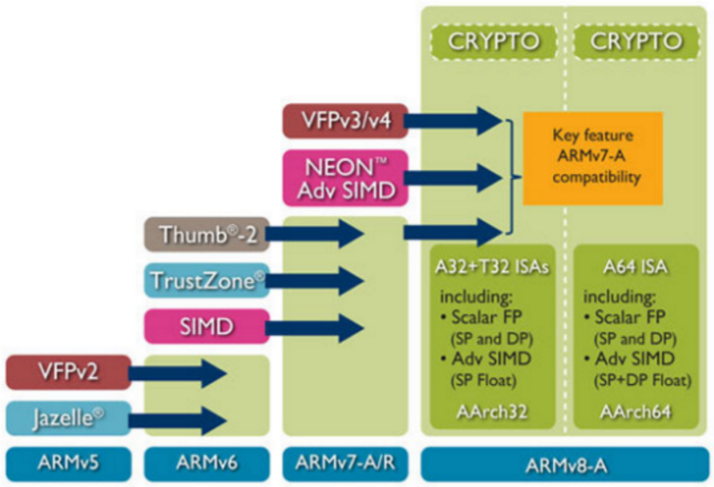
\includegraphics[width=.75\textwidth]{figuras/ref_001}
	\caption[Arquitetura ARM]{Arquitetura ARM: diferenças e semelhanças entre as arquiteturas ARMv5, ARMv6, ARMv7 e ARMv8-A, que mostra a compatibilidade das versões mais novas com as anteriores.} 
	\ Fonte: \cite{arm:2017:architecture}. 
	\label{figura:ref_001}
\end{figure}
A ARMv8-A tem sua arquitetura em 64 \textit{bits}, sendo compatível, portanto, com as versões 16 e 32 \textit{bits}. Além disso, a adição de instruções de 32 \textit{bits} permite, ainda, a otimização para requisitos emergentes. Um maior intervalo de endereçamento e instruções permitem a computação de novas categorias de aplicações para \textit{smartphones} e \textit{tablets}\footnote{\textbf{Texto original}: \textit{Increased availability of larger registers for general purpose and media instructions, a greater addressing range and cryptography instructions enable new categories of applications for superphone and tablet computing}.}. Outras características dessa arquitetura, descritas pela \citet{arm:2017:architecture}, que podem ser citadas, são:

\begin{enumerate}
	\item Registradores de uso geral de 64 \textit{bits}, SP (\textit{stack pointer}) e PC (\textit{program counter}).
	
	\item Processamento de dados de 64 \textit{bits} e endereçamento virtual estendido.
	
	\item Os estados de execução suportam três conjuntos de instruções principais:
	
	\begin{enumerate}
		\item AArch32: um conjunto de instruções de comprimento fixo de 32 \textit{bits}, aprimorado através das diferentes variantes de arquitetura;
		
		\item T32: (Thumb) introduzido como um conjunto de instruções de comprimento fixo de 16 \textit{bits}, posteriormente aprimorado para um conjunto de instruções de 16 e 32 \textit{bits} de comprimento misto na introdução da tecnologia Thumb-2;
		
		\item AArch64: é um conjunto de instruções de comprimento fixo de 64 \textit{bits} que oferece funcionalidade semelhante aos conjuntos de instruções ARM e Thumb.
	\end{enumerate}
	
\end{enumerate}

\section{Arquitetura x86}
\label{secao:arquitetura_x86}

Essa arquitetura teve seu nome (x86) originado do primeiro chip de 16 \textit{bits} da Intel, o 8086, que evoluiu para os modelos 80186, 80286, 80386 e 80486, todos com o sufixo "86",\ indicando a compatibilidade do conjunto de instruções com as versões anteriores. Inicialmente, essa arquitetura tinha seu conjunto de instruções do tipo CISC e, devido as necessidades do mercado, passou a utilizar instruções híbridas RISC/CISC. \cite{marmitt:2017:analise}. \citet{motyczka:2013:comparativo} explica que dessa forma "eles recebem instruções CISC, que são convertidas em instruções RISC para serem trabalhadas internamente buscando aperfeiçoar o processamento através do uso de \textit{pipeline}."\ São geradas micro operações parecidas com as instruções RISC, tendo-se assim uma máquina RISC dentro de uma x86. Mesmo sendo desenvolvido pela Intel, outras empresas passaram a utilizar a arquitetura x86 e, com o passar dos anos, esta se tornou padrão para computadores, notebooks e supercomputadores, sempre mantendo compatibilidades com as versões anteriores da arquitetura. A família x86 define um conjunto de tipos de instruções: movimentação de dados, aritmética e lógica, sequenciamento, manipulação de \textit{strings}, manipulação de \textit{bits}, suporte a linguagens de alto nível, entre outras.


\citet{mano:1993:computer} cita as principais características de processadores CISC:

\begin{enumerate}
	\item Número elevado de instruções (entre 100 e 250 instruções).
	
	\item Algumas instruções desempenham tarefas específicas e não são frequentemente utilizadas.
	
	\item Grande variedade de modos de endereçamento.
	
	\item Instruções com comprimento variável, assim utilizam diferentes números de \textit{bits} para codificar as instruções que dependem: quantidade de entradas da instrução, modos de endereçamento utilizados, entre outros fatores. \cite{lorenzoni:2012:analise}.
\end{enumerate}		


\section{Sistemas Embarcados}
\label{secao:sistemas_embarcados}

Os sistemas embarcados, também conhecidos como sistemas embutidos, são definidos como sistemas computacionais para uso específico ou dedicados. Estes estão se tornando cada vez mais populares e presentes na vida humana, principalmente por causa de algumas de suas vantagens, tais como: economia de energia, portabilidade, complexidade de processamento e baixo custo. A computação ubíqua - que diz respeito ao suporte computacional contínuo e permanente ao ser humano - tem como base os sistemas embarcados. Os núcleos de processamento de sistemas embarcados podem ser de propósito geral - que disponibilizam no hardware várias funções já implementadas, executam as mais variadas aplicações e funcionam com a execução de um programa - na qual tarefas como buscar, decodificar e executar instruções afetam diretamente o desempenho; ou podem ser de uso específico, possuindo circuitos integrados que são desenvolvidos para um conjunto específico de funções (ASIC - \textit{Aplication Specific Integrated Circuit}). \cite{cruz:2013:desenvolvimento}.

Os projetos de sistemas embarcados podem apresentar uma grande flexibilidade não apenas do ponto de vista da programação (software), mas também em relação à parte física (hardware), especialmente quando implementados em sistemas reconfiguráveis. Hardware específico ou dedicado, normalmente, é separado para tarefas que exigem alto poder de processamento, assim as demais funcionalidades são implementadas por meio de software \cite{wei:2008:research}.
Essa característica faz com que os sistemas de uso específico apresentem um desempenho melhor (na execução de tarefas) do que os sistemas de propósito geral.

\section{Raspberry Pi}
\label{secao:raspberry_pi}

É um pequeno computador que possui memória primária e secundária, CPU (unidade central de processamento), GPU (unidade de processamento gráfico), sistema operacional (SO), conectores USB (\textit{Universal Serial Bus}), saída de vídeo, saída de áudio, interface \textit{Ethernet}, entre outros. Possui baixo custo e possibilidade de aplicação em problemas reais. Possui, ainda, pinos (GPIO – \textit{General Purpose Input/Output}) que possibilitam o recebimento e o envio de sinais elétricos. \cite[p.~3]{sheid:2015:raspberry}. 
\citet[p.~19]{coutinho:2016:sistema} afirma que “desenvolvida pela fundação Raspberry Pi, no Reino Unido, a plataforma Raspberry é um computador de baixo custo, pequeno, \textit{Open Source} e com interfaces para vários periféricos.” A \citet{fundacaoraspberry:2017:raspberry} define esta placa como "um pequeno computador capaz de ser usado em projetos eletrônicos, e para muitas das coisas que seu PC de mesa faz, como planilhas, processamento de texto, navegar na internet e jogar. Ele também reproduz vídeo de alta definição." Suas principais características são:

\begin{enumerate}
	\item 1.2GHz 64-\textit{bits quad-core} ARMv8-A CPU com memória \textit{cache} de 32kB nível 1 e 512kB nível 2.
		
	\item 1GB RAM LPDDR2 (900 MHz).
		
	\item 4 portas USB 2.0.
		
	\item 40 pinos GPIO.
		
	\item Porta \textit{Full} HDMI.
		
	\item Porta 10/100 \textit{Ethernet}.
		
	\item \textit{Combined} 3.5mm \textit{audio jack and composite video}.
		
	\item Interface de câmera (CSI).	
	
	\item \textit{Display} interface (DSI).
		
	\item Slot para cartão Micro SD (agora \textit{push-pull}, em vez de \textit{push-push}).
		
	\item VideoCore IV (Núcleo gráfico 3D) - suporte a OpenGL ES 2.0, acelerador de hardware OpenVG, alta capacidade de codificação e decodificação em perfil 1080p30 H.264. A GPU tem capacidade de 1Gpixel/s, 1.5Gtexel/s ou 24GFLOPs em processamento de propósito geral e apresenta várias filtragens de texturas,  além de infra-estrutura DMA (\textit{Direct Memory Access})\footnote{\textbf{Texto original}: \textit{VideoCore IV 3D graphics core - The GPU provides OpenGL ES 2.0, hardware-accelerated OpenVG, and 1080p30 H.264 high-profile encode and decode. The GPU is capable of 1Gpixel/s, 1.5Gtexel/s or 24 GFLOPs of general purpose compute and features a bunch of texture filtering and DMA infrastructure}.}.
	 	
	\item Completa compatibilidade com os Raspberry Pi 1 e 2. A Figura \ref{figura:ref_002} apresenta a distribuição dos componentes na placa e a Tabela \ref{tabela:consumo_raspberry} apresenta os dados necessários para a alimentação da placa. Os pinos GPIO podem fornecer até 50mA com segurança (note que isso significa que 50mA distribuídos em todos os pinos: um pino individual GPIO só pode seguramente fornecer até 16mA).
\end{enumerate}	

\begin{figure}[htb]  
	\centering
	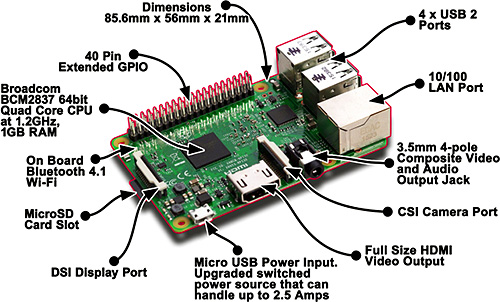
\includegraphics[width=.8\textwidth]{figuras/ref_002}
	\caption[Raspberry Pi 3 Modelo B]{Componentes da Raspberry Pi 3 Modelo B, sendo estes de entrada e saída (gpio, ethernet, USB, HDMI, interface CSI e DCI, conector áudio, conector fonte de energia, slot SD card), bluetooh 4.1 e Wi-Fi.}
	\ Fonte: \cite{fundacaoraspberry:2017:raspberry}.
	\label{figura:ref_002}
\end{figure}

\begin{table}[htb] \centering
	\caption{Modelos e características da raspberry, sendo capacidade recomendada de alimentação, corrente máxima consumida pelos periféricos USB e o consumo de corrente ativa típico na placa.} \label{tabela:consumo_raspberry}
	\begin{tabular}{c|ccc}        \hline
		& \textbf{Capacidade}  & \textbf{Corrente máxima} &   \textbf{Consumo de}    \\ 
		\textbf{Raspberry Pi} &   \textbf{recomendada da}    & \textbf{consumida pelos} & \textbf{corrente ativa}  \\
		& \textbf{fonte de alimentação} & \textbf{periféricos USB} & \textbf{típico na placa} \\ \hline \hline          
		Model A 	 &        700mA         &     500mA       &      200mA      \\ 
		Model B	 	 &	      1,2A          &      500mA      &      500mA      \\ 
		Model A+ 	 &        700mA         &      500mA      &      180mA      \\ 
		Model B+ 	 &        1,8A          &   600mA/1,2A    &      330mA      \\  
		&                      &(\textit{switchble}) &             \\ 
		2 Model B	 & 	      1,8A          &   600mA/1,2A    &        -        \\  
		&                      &(\textit{switchble}) &             \\ 
		3 Model B	 &  	  2,5A          &      1,2A       &      ~400mA     \\ 
		Zero W		 &   	  1,2A          &\textit{Limited by} &      150mA   \\ 
		&                      &\textit{PSU only} &                \\
		Zero		 &        1,2A          &\textit{Limited by}&      100mA    \\ 
		&                      &\textit{PSU only} &                \\ \hline
	\end{tabular}
	\\ Fonte: \cite{fundacaoraspberry:2017:raspberry}.
\end{table}

\citet[p.~20]{coutinho:2016:sistema} afirma  que “existem várias versões diferentes de sistemas operacionais (SOs) compatíveis com a plataforma, sendo que o SO do Raspberry é instalado no cartão SD do dispositivo.” Para fins de uso não específico da placa, é recomendado a utilização da distribuição Linux Raspbian, recomendação esta feita pela fabricante que ainda acrescenta: “Raspbian é um sistema operacional livre baseado no Debian, otimizado para o hardware Raspberry Pi. Raspbian vem com mais de 35.000 pacotes: software pré-compilado empacotado em um formato agradável para fácil instalação em seu Raspberry Pi.” \cite{fundacaoraspberry:2017:raspberry}.  

\section{Algoritmo Genético}
\label{secao:AG}

Os Algoritmos Genéticos (AGs) são uma técnica de Inteligência Artificial baseada no princício da seleção e evolução natural de orgamimos biológicos (Darwinismo) em que os indivíduos que mais se adaptarem ao ambiente terão mais chance de sobreviver e se reproduzirem. Os AGs são amplamente aplicados em busca e otimização de resultados (buscam a melhor solução para um determinado problema). (\cite{pacheco:1999:algoritmos}. \cite{silva:2001:otimizacao}). 

Um AG trabalha de forma aleatória mas orientada para algumas regras probabilísticas, de acordo com os mecanismos de reprodução e genética natural. Primeiro, cria-se uma população inicial (em que cada indivíduo é uma solução para o problema). Esta população é então avaliada para se conhecer quais são os melhores indivíduos (com melhor \textit{fitness} ou melhor aptidão). Estes devem ter maiores chances de cruzamento para que se garanta a reprodução e propagação do material genético para as proximas gerações. Algumas estratégias sugerem passar os melhores indivíduos direto para o proxima geração. Os indivíduos são implementados de forma que as características possam ser trocadas com outros indivíduos, tendo-se, assim, a reprodução. Cruzando-se os indivíduos, gera-se uma nova população que deve ser do mesmo tamanho da população inicial, a população antiga é substituida, então, por esta nova. De forma percentual e aleatória, aplica-se a mutação sobre a população (alteração dos cromossomos pode gerar indivíduos melhores). Esses procedimentos são repeditos até que se tenha uma solução aceitável ou até que se atinja um número máximo de gerações. A Figura \ref{figura:ref_007} mostra um fluxograma básico e o Algoritmo \ref{algoritmo:ag} apresenta o pseudocódigo básico de um AG. (\cite{holland:1992:adaptation} e \cite{goldberg:1989:genetic} apud \cite{avila:2002:algoritmos}).

\begin{figure}[htb]  	
	\centering	
	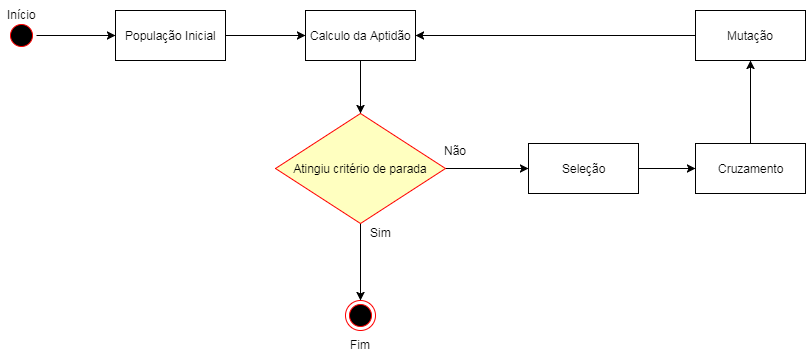
\includegraphics[width=\textwidth]{figuras/ref_007}
	\caption[Fluxograma de um AG]{Fluxograma de um AG básico, que gera população inicial aleatoriamente, avalia esta população, verifica o critério de parada, faz a seleção dos melhores indivíduos, realiza o cruzamento (o que gera nova população), realiza a mutação e volta ao critério de parada. Caso não tenha sido atingido, o algoritmo volta ao passo de seleção e, assim continua até que se satisfaça o critério de parada.} 	
	\label{figura:ref_007}
\end{figure}

\begin{algoritmo}[!htb]
	\begin{algorithmic}[1]
		\\$gerac \leftarrow 0$;    //inicializa contador gerações
		\\$Pop(gerac) \leftarrow Inicializa\_populacao()$;    //população inicial gerada aleatoriamente
		\State$Avalia(Pop(gerac))$;    //avalia população inicial
		\Repeat 
			\State$ P \leftarrow Seleciona(Pop(gerac)) $;    //seleciona indivíduos para cruzamento
			\State$ P \leftarrow cruzamento(P) $;    //cruzamento ou recombinação dos indivíduos
			\State$ P \leftarrow mutacao(P) $;    //operação de mutação nos indivíduos
			\State$ gerac \leftarrow gerac + 1 $;    //incrementação do contador de gerações
			\State$ Pop(gerac) \leftarrow atualiza(P)$; //atualiza a população atual
			\State$ Avalia(Pop(gerac))$; // avalia população atual
		\Until      //satisfaça condição de parada
		\\Print(Avalia(Pop(gerac)));
	\end{algorithmic}
	\caption{Pseudocódigo do AG clássico} \label{algoritmo:ag}
\end{algoritmo}

Os indivíduos devem possuir cromossomos, sendo que estes devem ter genes que são caracterésticas ou informações sobre os indivíduos. Em outras palavras é o material genético do indivíduo que será trocado com outros indivíduos durante o cruzamento. Sendo assim, faz-se necessário uma função que seja capaz de avaliar o \textit{fitness} dos indivíduos. A codificação do indivíduo e da função de avaliação tem grande importância, pois possui a responsabilidade de relacionar o algoritmo com o problema real, avaliando quão boas são as características dos indivíduos em relação ao problema. \cite{neto:2011:computaccao}.

\section{O Problema do Caixeiro Viajante}
\label{secao:caixeiro_viajante}

O Problema do Caixeiro Viajante (PCV, do inglês: \textit{Traveling Salesman Problem} - TSP) é um dos mais conhecidos problemas de otimização combinatória. Basicamente, consiste no problema de encontrar a melhor rota possível (que pode ser menor caminho, caminho de menor custo, entre outros) em um conjunto de cidades, sendo que cada cidade só pode ser visitada uma única vez no trajeto. Quando o percurso entre duas cidades (ou nós) x e y não sofre interferência do sentido (Pxy = Pyx), o PCV é chamado de simétrico; quando há diferença em virtude do sentido do trajeto, é chamdo de PCV assimétrico. O simétrico é, em geral, mais difícil de ser resolvido que o assimétrico. O PCV "tem sido usado como \textit{benchmark} para avaliação de novos algoritmos e estratégias de solução que envolvem busca tabu, algoritmos genéticos, \textit{simulated annealing}, redes neurais artificiais, entre outras." \cite{cunha:2002:experimentos}. O estudo e aplicação do PCV não se restringe ao cenário de desempenho computacional, mas está presente em inúmeras áreas (pesquisa operacional, matemática, física, biologia, inteligência artificial, entre outros) em vários tipos de problemas reais, como por exemplo, roteirização de veículos e \textit{design} de circuitos.

\begin{citacao}
	Sob a ótica de otimização, o PCV pertence à categoria conhecida como NP-difícil (do inglês NP-\textit{hard}), o que significa que possui ordem de complexidade exponencial. Em outras palavras, o esforço computacional para a sua resolução cresce exponencialmente com o tamanho do problema (dado pelo número de pontos a serem atendidos). \cite{cunha:2002:experimentos}.
\end{citacao}

Problemas dessa categoria não podem ser resolvidos de maneira ótima em tempo viável, assim as técnicas atuais para resolução são conhecidas como heurísticas, pois não garantem um resultado ótimo, mas sim um resultado aproximado. Segundo \citet{helsgaun:2000:effective}, as heurísticas para resolução do PCV podem ser implementadas de duas formas:

\begin{enumerate}
	\item Métodos de contrução de roteiros: os nós ou cidades são inseridos no roteiro de forma gradual e sequencial, sem que a solução parcial seja avaliada e/ou melhorada, assim a sequencia é montada e não é alterada mais.  
	
	\item Métodos de melhorias de roteiros: através de um roteiro já obtido, com alguma técnica, busca-se melhorar o roteiro (diminuir o custo ou a distância do trajeto, por exemplo). Há autores que consideram uma terceira forma, que une a técnica de construção e a de melhoria de trajeto. \cite{cunha:2002:experimentos}.
\end{enumerate}

Segundo \citet{laporte:2000:classical} e \citet{reinelt:1994:traveling}, a construção de roteiros pode ser dada através:

\begin{enumerate}
	\item método do vizinho mais próximo;	
	\item método da inserção;	
	\item método das economias;	
	\item heurísticas baseadas em árvores de cobertura (\textit{spanning trees}). \cite{cunha:2002:experimentos}.
\end{enumerate}

\section{Sistemas Paralelos}
\label{secao:sistemas_paralelos}

Sistema paralelos são do tipo MIMD (\textit{Multiple Instruction, Multiple Data}), pois possuem múltiplos fluxos de instruções e múltiplos fluxos de controle, como os processadores \textit{multicore}, os computadores com múltiplos processadores e os \textit{clusters}. O termo \textit{multicore} é usado para definir sistemas com vários núcleos em um único chip e também sistemas com núcleos em chips separados ou independentes. Nos sistemas com mais de um núcleo que compartilham memória, o gerenciamento e sincronismo da mesma torna-se ainda mais rigoroso para evitar inconsistências nos dados. Para que os recursos implementados por sistemas paralelos sejam realmente utilizados, os softwares que são executados nos mesmos devem ter suporte para essas arquiteturas. Para isso, os algoritmos devem ter três características básicas: distribuição das tarefas para os diferentes processadores (mapeamento), execução compartilhada das tarefas conforme a dependência de dados (compartilhamento) e identificação dos dados que trafegam entre os processadores (identificação). \cite{lima:2016:implantacao}. 

\citet{hwang:1987:advanced} sugere que há diferentes níveis de paralelismo, sendo estes:

\begin{enumerate}	
	\item Nível 5: processos (\textit{jobs}) e programas independentes;
	\item Nível 4: sub-processos e pontes de programas;
	\item Nível 3: rotinas, sub rotinas e co-rotinas;
	\item Nível 2: iterações (\textit{loosp});
	\item Nível 1: instruções (\textit{pipeline}). \citet{navaux:1989:introducao}.
\end{enumerate}

O nível mais alto é o algorítmico e o inferior (de instruções) é implementado em hardware - quanto mais baixo o nível mais fina é a granularidade do processamento. O paralelismo explora um ou a combinação desses níveis e a tendência é de que quanto mais destes níveis implementados na mesma máquina, mais poderosa esta será. Alguns autores sugerem que há também:

\begin{enumerate}
\item Paralelismo em nível de \textit{bit} (\textit{bits} de uma instrução são processados em paralelo).
	
\item Paralelismo em nível de dados (dados são acessados em paralelo e seus resultados são combinados).

\item Paralelismo em nível de tarefas (fluxos de controle independentes para cada tarefa).
\end{enumerate}

\section{Biblioteca OpenMP}
\label{secao:openmp}

É uma biblioteca desenvolvida para processamento paralelo de algotimos utilizando memória compartilhada, em que através de diretivas de compilação, rotinas da biblioteca e variáveis de ambiente tem-se a paralelização do algoritmo de forma que o código sequencial é minimamente modificado e, por ser de memória compartilhada, as \textit{threads} comunicam-se através de variáveis compartilhadas. \cite{rodrigues:2012:proposta}.

O uso desse tipo de variável exige um controle de acesso rigoroso para evitar problemas com inconsistência nos dados ou resultados errôneos. Há a implementação de uma política de acesso para que, enquanto uma \textit{thread} realizar a escrita, nenhuma outra possa ler ou escrever na variável em questão - fazendo com que as demais que necessitem acessar entrem em estado de espera (este problema é conhecido como \textit{race condition} ou condição de corrida). Já o processo de leitura pode ser feito simultaneamente por todas as \textit{threads} do perocesso. \cite{openmp:2011:application}. 

Contudo, quanto menor for o uso de variaveis compartilhadas e menor for a dependência entre as \textit{threads}, melhor será o desempenho do algoritmo. Dessa forma, diminui-se gargalos causados por acessos ou pela espera dos acessos a estas variáveis. \cite{rodrigues:2012:proposta}.

\chapter{Revisão de Literatura}

\citet{ramos:2016:avaliacao}  avaliaram um \textit{cluster} formado com 16 placas Raspberry Pi, totalizando 64 núcleos e 16GB de memória RAM – memória secundária de 16GB (cartão SD), SO Raspbian, interface de rede de 100Mb/s e todas as placas interligadas por um \textit{switch ethernet} de 100Mb/s com 24 portas, para análise de imagens microscópicas. Essa avaliação compara processadores de baixo custo com CPUs multicores considerando tempo de execução, gasto energético, custo dos equipamentos e performance do \textit{cluster}. Cada raspberry (modelo 2B) possuia: processador Quad Core ARM7 Cortex 900MHz, 1GB RAM, interface de rede 100Mbits/s. Para instalação do SO foram utilizados cartões micro SD 16GB classe 10 (até 80MB/s). O \textit{cluster} foi construído em quatro torres contendo quatro placas em cada e cada fonte de energia (de 5V DC e 2A) alimentou duas placas. Foi utilizada linguagem C++ e a paralelização foi feita utilizando a biblioteca MPI. A execução foi no modelo mestre/escravo. Foram utilizadas como entrada para os testes 512 imagens de 1K x 1K pixels, totalizando 6GB de dados de entrada. Conclui-se que em consumo de energia, a placa (em capacidade máxima de processamento) obteve consumo menor que os computadores (mesmo em estado ocioso: apenas as aplicações do sistema), chegando a 2x menos energia. O \textit{cluster} custou mais caro que os PCs, porém em desempenho ele foi 2x mais rápido que a máquina com processador I7 e 10x mais rápido que a máquina com processador Core2Duo, tornando o \textit{cluster} mais eficiente. Nas avaliações das máquinas, em comparação com uma placa Raspberry Pi, esta apresentou desempenho pior que das máquinas (I7 e Code2Duo). Devido as memórias (primárias e secundárias) da placa serem mais lentas que as dos PCs, operações que realizam muitos acessos as essas memórias fazem com que o desempenho da Raspberry caia se comparado ao dos PCs (por exemplo: operações que visitam muitos pixels vizinhos do ponto analisado dentro de uma imagem). O processamento das imagens se deu pelas seguintes etapas: normalização, segmentação, extração de características, sumarização das características e clusterização.

\citet{lima:2016:implantacao} propôs a análise de desempenho de um \textit{cluster} embarcado de baixo custo composto por processadores da arquitetura ARM e plataforma Raspberry Pi. O trabalho analisava o impacto de usar as bibliotecas MPICH-2 e OpenMPI, executando os programas dos \textit{benchmarks}  HPCC e HPL, a fim de verificar qual implementação obteve um melhor desempenho e um baixo consumo de energia. Os resultados de desempenho e consumo de energia do \textit{cluster} com esses programas mostraram que é possível usar \textit{clusters} de plataformas embarcadas de baixo custo e tendo \textit{speedups} e consumo de energia satisfatórios. 

\citet{godoi:2015:estudo}  apresentou uma comparação de custo/benefício entre um \textit{cluster} de computadores \textit{desktop} tradicionais (computadores HP Compaq 6005 Pro Microtower) e de dispositivos de baixo consumo de energia, como Raspberry Pi Modelo, B e Cubietruck. Para testá-los, foram implementados algoritmos (multiplicação de matrizes MxN e Caixeiro Viajante) para resolução de problemas das classes P e NP-Difícil além do software \textit{benchmark} HP Linpack (HPL). A biblioteca MPI foi utilizada para troca de mensagens. Três \textit{clusters} homogêneos (no formato mestre/escravo) foram montados: computadores \textit{desktop}, Raspberry Pi e Cubietruck. Foram realizadas análises para se obter dados de custo energético (foi desenvolvido um sistema com microcontrolador Tiva e um sensor de corrente), financeiro e velocidade de processamento (para esse parâmetro utilizou-se \textit{speedup} e o \textit{benchmark} HPL). Com os dados coletados de ambos os clusters, foi possível estimar o custo e benefício gerado, bem como verificar sua aplicabilidade. Concluiu-se que os clusters de Raspberry Pi e de Cunietruck têm custo financeiro e consumo energético muito inferior ao de computadores \textit{desktops}. Porém, ao analisar os dados de \textit{speedup} e do HPL, pode-se perceber que a capacidade de processamento do cluster de computadores desktop é superior ao demais. Por fim, concluiu-se, também, que cluster de dispositivos ARM são recomendados para aplicações que necessitam de baixo custo e baixo consumo energético, já cluster de computadores desktops são recomendados para aplicações em que o tempo seja crítico ao sistema e não haja preocupação com custo e consumo (inclusive de refrigeração).

\citet{erckumecka:2015:avaliacao} realizaram a construção de dois \textit{clusters} isolados um do outro: um com sete computadores HP Compaq 6005 Pro Microtower e outro com oito dispositivos ARM (Raspberry Pi), modelo B. Os computadores com distribuição Linux Ubuntu Server e Raspbian para os dispositivos ARM. A biblioteca MPI foi utilizada para a paralelização. Como parâmetros de análise, foram considerados o \textit{benchmark} HP Linpack (HPL), calculo de \textit{speedup}, consumo de energia e custo monetário dos equipamentos. Os cálculos de speedup serão realizados a partir de algoritmos projetados para solucionar problemas, como: \textit{Quick-Sort}, multiplicação de matriz e Caixeiro Viajante utilizando o método GRASP (\textit{Greedy Randomized Adaptive Search Procedure}). Para cálculo do consumo energético foram utilizados sensores de corrente e tensão. Conclui-se que é possível utilizar técnicas de paralelização para equilibrar a inferioridade dos dispositivos embarcados em relação aos computadores convencionais. Sendo assim, é possível criar um sistema computacional distribuído de alto poder de processamento e baixo custo, tanto monetário, quanto energético. Contudo, os dados obtidos após a avaliação mostraram que o \textit{cluster} de Raspberry Pi é inviável para grandes cargas de processamento e com poucos nós.

\citet{nunes:2014:analise} compararam o desempenho de sistemas reais e sistemas emulados em dispositivos com recursos limitados, nesse caso o Raspberry Pi. A análise de desempenho foi realizada em serviços \textit{web} configurados na placa Raspberry Pi (utilizando RESTful e o \textit{framework} CXF) – foram considerados os tempos de processamento de requisições, de empacotamento e desempacotamento de mensagens. Para avaliar o desempenho dos serviços \textit{web}, o seguinte cenário foi proposto: a aplicação cliente gerava uma sequência aleatória de números, enviava para o servidor, que então recebia a mensagem, ordenava esses números e então os enviava de volta ao cliente. Ordenados e após serem recebidos, a aplicação cliente finalizava a conexão com o servidor. Foi utilizado um Raspberry Pi, modelo B com cartão SD de 16GB e SO Linux Raspbian. Para o sistema emulado, foi utilizado o software Qemu, que simulou um hardware equivalente ao do Raspberry e com o mesmo SO. Os experimentos foram realizados 50 vezes (IC de 95\%) com mensagens de 100Kb e 500Kb tanto no sistema real quando no emulado. Uma solução foi implementada para obter tempo de serialização e deserialização e tempo total das aplicações tanto no cliente como no servidor. Conclui-se  que o comportamento no sistema emulado e no sistema real são próximos tanto no cliente como no servidor. No sistema emulado há um leve aumento nos tempos, mas é justificado devido ao custo da emulação.

\citet{crotti:2013:raspberry} propuseram um sistema para acesso remoto utilizando uma placa Raspberry Pi. Foi configurado um servidor \textit{web} na placa que se comunicava com uma pagina \textit{web} (que estava na mesma rede). Através dessa página foi possível o gerenciamento de portas (envio de comandos, acionamento e/ou leitura de portas etc) para o servidor \textit{web} na placa. Também foi configurado uma \textit{webcan} que monitorava os experimentos, isto é, as imagens eram envidas para a placa e esta as enviavam para a internet (\textit{streaming} de vídeo). Foi configurado na placa: pacote lighttpd (um servidor \textit{web}) para servidor de arquivos em C e também PHP, pacote Moiton para o servidor de câmeras (em que cada câmera recebia uma porta de endereço). Na página \textit{web}, foram colocados três botões (acender, apagar e verificar o estado de um LED), além de um quadro que exibe o \textit{streaming} da \textit{webcan}. Cada um desses botões enviava comandos de leitura de arquivos (.C) específicos localizados no servidor de arquivos. Em cada um desses arquivos continham as rotinas e as funções (acender, apagar e verificar).  Observa-se que a aplicação proposta obteve ótimos resultados, inclusive da utilização do Raspberry como servidor, o que possibilita a criação de servidores \textit{web} de baixo custo porém com bom desempenho.

\citet{silva:2012:avaliacao} apresentaram uma implementação do Problema do Caixeiro Viajante na estrutura de um AG de forma paralela utilizando a biblioteca OpenMP e a biblioteca Pthreads. Nessa implementação do AG, cada combinação de rota (passando por todas as cidades) foi definida como um indivíduo, e um conjunto desses indivíduos uma população; cada nó (ou cidade) foi definido como um gene. Assim, quanto maior a população, maior a chance de encontrar uma boa rota, porém maior será o processamento necessário para gerar a próxima geração. Foram gerados conjuntos de populações (ou ilhas) que sofrem a mutação uma independente da outra (a função que realiza a mutação é executada de forma paralela, ou seja, as ilhas sofrem mutações ao mesmo tempo, porém independentes umas das outras). A implementação foi feita em C e cada indivíduo foi representado por um vetor com tamanho igual ao número total de cidades (as coordenadas das cidades estavam em um vetor estático de ponto flutuante também com tamanho igual ao número de cidades) - a população é um vetor de indivíduos. Na implementação, usando a biblioteca pthreads, cada \textit{thread} ficou com uma \textit{struct} e nela havia um vetor de indivíduos (ou população), sendo possível ter as ilhas isoladas umas das outras (pois cada {thread} só acessa sua \textit{struct}). Os testes foram realizados em dois computadores ambos com a mesma distribuição Linux, um com quatro núcleos reais e outro com dois reais (em que cada núcleo real simula dois núcleos lógicos: tecnologia SMP - \textit{Symmetric Multi-Processor}). Foram ajustados: taxas de erro, número máximo de gerações, número de indivíduos em cada população e número de indivíduos na elite. Os resultados mostraram, que no computador com SMP, a implementação com OpenMP obteve melhor resultado que a pthread, enquanto que no computador com quatro núcleos reais, a pthread obteve melhor resultado. Nos dois casos, a implementação paralela obteve resultado significativamente melhor em relação a sequencial. Apesar de que nos cenários propostos a implementação paralela foi melhor que a sequencial, deve-se tomar cuidado ao escolher entre as bibliotecas openMP e pthread, pois cada uma apresentou desempenho melhor em diferentes situações, tornando essencial a análise do problema antes da escolha.

Este trabalho se difere dos demais ao comparar o desempenho com um \textit{notebook} ao invés do computador de mesa e não levar em consideração o consumo de energia. Outra diferença está nas métricas de desempenho utilizadas ($Sd$ e $Ef$, como é apresentado na Seção \ref{secao:metricas}) e a não utilização de aplicações do tipo \textit{benchmark} para análise.

\chapter{Materiais e Métodos}

Este capítulo apresenta os materiais utilizados para o desenvolvimento, os métodos aplicados e as métricas selecionadas para a análise do desempenho com base nos resultados obtidos.

\section{Materiais}
\label{secao:materiais}

Para a realização deste trabalho, foi utilizado: 
\begin{enumerate}
	\item \textit{Notebook} Asus X44C com sitema operacional Linux Ubuntu 16.04 professional 64 bits. Suas especificações são apresentadas no Quadro \ref{quadro:notebookasus}.
	
	\item placa Raspberry Pi 3B com cartão MicroSD de 16GB. Suas especificações são apresentadas na Seção \ref{secao:raspberry_pi}.
	
	\item Compiladores GCC e G++ versões 5.4.0.
	
	\item Biblioteca OpenMp 3.1.	
\end{enumerate}

\begin{quadro}[htb] \centering
	\begin{tabular}{ll}        \hline
		\textbf{Item}		 & \textbf{Descrição}						  \\ \hline \hline
		Modelo               & \textit{Notebook} Asus X44C                \\ 
		Processador          & Intel Core i3-2330M 2.2GHz                 \\ 
		Memóra               & 4 GB DDR3 1333MHz SDRAM \textit{On-board}  \\ 
		Sistema Operacional  & Linux Ubuntu 16.04 LTS - 64 \textit{bits}  \\ 
		Armazenamento        & HD SATA 500 GB - 5400 rpm                  \\ 
		Fonte de Alimentação & Input: 127/220 V AC, 50/60Hz               \\
		& Output: 19V DC, 3,42A, 65W                 \\ \hline
	\end{tabular}
	\caption{Especificações de hardware (processador, memória, HD, alimentação etc.) do \textit{Notebook} Asus X44C usado no desenvolvimento deste trabalho.}
	\ Fonte: \cite{asus:2017:x44c}.
	\label{quadro:notebookasus}
\end{quadro}

\subsection{O Algoritmo}
\label{secao:oalgoritmo}

O algoritmo escolhido foi um AG paralelo para resolução do PCV disponibilizado por \citet{arora:2017:travelling}. O mesmo foi escolhido devido a sua granularidade e grande capacidade de paralelização conciliado com a grande carga de processamento que consegue exercer sobre o hardware. Os arquivos de entrada para o algoritmo, possuíam três colunas. A primeira era um número inteiro que representava a cidade, a segunda e a terceira eram, respectivamente, a coordenada X e Y das cidades (sendo estes números inteiros entre 0 e 10000, gerados aleatoriamente). O algoritmo, primeiramente, armazenou o tempo atual. Posteriormente realizou a leitura do arquivo de entrada e criou uma matriz com as coordenadas X e Y das cidades. Em seguida, foi gerada uma matriz de distância das cidades. Esta era a distância euclidiana, que em um espaço bi-dimensional (entre os pontos $P=(p_1,p_2,...,p_n)$ e $Q=(q_1,q_2,...,q_n)$) é dada pela Equação \ref{equacao:deuclid}. 

\begin{equation} \label{equacao:deuclid}
d(P,Q) = \sqrt{\sum_{i=1}^{n}(p_i-q_i)^2}
\end{equation}

Na sequência foi gerada aleatoriamente a população inicial. O algoritmo mantinha também os 10 melhores cromossomos (impedindo a extinção dos mesmos) de todas as gerações para propagá-los de tempos em tempos. O Código \ref{codigo:pos_leitura_entrada} mostra a sequência de instruções executadas após a leitura do arquivo de entrada.

\begin{codigo}[!htb]
	\begin{Verbatim}
int N1 = ((10*N*N)>10000)?10000:(10*N*N);			

//Conjunto completo de cromossomos
vector< vector<int> > chromos(N1, vector<int> (N,0));  

//Conjunto dos melhores cromossomos
vector< vector<int> > bests(BESTS, vector<int> (N,0)); 

int best = 0;
vector<float> fitness(N1,2000000000.0);                
float maxfitness = 2000000000.0;	//distância máxima					
omp_lock_t locks[N1],lock4bests;

//Bloqueio de inicialização para acessar a matriz
omp_init_lock(&lock4bests);	
	
for(i = 0;i<N;i++){	//gerando população inicial
	chromos[0][i] = i;
}
	\end{Verbatim}
	\caption{Instruções executadas após a leitura do arquivo de entrada.} \label{codigo:pos_leitura_entrada}
\end{codigo}

Até nesse momento, o código era executado de forma sequencial. O trecho de início da paralelização é mostrado no Código \ref{codigo:paralelizacao}, em que o comando $\#pragma$ $omp$ $parallel$ definia a paralelização e os comandos $shared$ e $private$ definiam, respectivamente, as variaveis compartilhadas e as que não eram, entre as \textit{threads} criadas. Pode-se notar, também, a aleatorização e o cálculo do \textit{fitness} dos cromossomos da população inicial.

\begin{codigo}[!htb]
	\begin{Verbatim}
#pragma omp parallel shared(fitness,maxfitness,best,chromos,
locks,lock4bests,N,N1,dist,bests) private(GREEDY,MUTATE)
{
	NUMT = omp_get_num_threads();
	cout<<NUMT<<endl;
	#pragma omp for
	for(int il = 0 ; il<N1;il++){
		omp_init_lock(locks+il);
		chromos[il] = chromos[0];

		// Aleatorizando a população inicial
		random_shuffle(chromos[il].begin(), chromos[il].end(),myrandom);
		float x=0;
		
		//\textit{fitness} da população inicial								
		for(int j = 0 ; j<N;j++){
			x+=dist[chromos[il][j]][chromos[il][(j+1)%N]];
		}
		fitness[il] = x;
		if(maxfitness>fitness[il]){

			//Atualizando o conjunto 
			//dos melhores cromossomos
			omp_set_lock(&lock4bests);  
			maxfitness = fitness[il];		
			best = (++best)%BESTS;
			bests[best] = chromos[il];
			omp_unset_lock(&lock4bests);
		}

	}
	\end{Verbatim}
	\caption{Rotina de paralelização do AG.} \label{codigo:paralelizacao}
\end{codigo}

O máximo de gerações foi de 100000, sendo que nas 8000 (80\%) primeiras gerações a taxa de mutação era de 20\% e nas 2000 (20\%) restantes a taxa de mutação aumentava para 40\%. O Código \ref{codigo:inicio_geraceos} apresenta o laço $for$ que executava as gerações, definição das taxas de mutação e a propagação dos melhores cromossomos na população atual.

\begin{codigo}[!htb]
	\begin{Verbatim}
int iterations; 
	
//inicio da execução das gerações 
for(iterations = 0 ; iterations < MAX_ITERS; iterations++){
	GREEDY = (int)(100- (((float)iterations)/MAX_ITERS)*10);
	
	//configuração das taxas de mutação (20\% e 40\%)      
	MUTATE = (iterations<((4*MAX_ITERS)/5))?20:40;
	#pragma omp master                                            
	{
	//imprimindo maior fitnees geração atual									
	if((iterations%1000==999)||(iterations%1000==0))cout<<
	iterations<<" ~ "<<GREEDY<<" ~ "<<MUTATE<<" ~ "
	<<maxfitness<<endl;
	}
	#pragma omp for nowait
	for(int nb = 0;nb<BESTS;nb++){    		
		int te = rand()%N1;
	
		//Semeando os melhores cromossomos				
		omp_set_lock(locks+te);
		chromos[te] = bests[nb];
		omp_unset_lock(locks+te);	
	}
	\end{Verbatim}
	\caption{Rotina de execução das gerações.} \label{codigo:inicio_geraceos}
\end{codigo}

Haviam disponíveis quatro métodos diferentes de cruzamento dos cromossomos - \textit{Partially Mapped Crossover} (PMX), \textit{Greedy Crossover} (GX), \textit{Cycle Crossover} (CX) e \textit{Edge Recombination Crossover} (ERX) - em que, a cada geração, era sorteado aleatoriamente um desses. O Código \ref{codigo:cruzamento} mostra como era feita a seleção do método de cruzamento e a aplicação da mutação nos cromossomos. O Código \ref{codigo:avalizao} mostra o cálculo do \textit{fitness} da população atual e a atualização do conjunto dos melhores indivíduos.

\begin{codigo}[!htb]
	\begin{Verbatim}
int select = (rand()%101),index,temp;
			
// Seleção da técnica de cruzamento	
if(select<GREEDY)gx(chromos[first],chromos[second],dist);	
else if(select<GREEDY+PMX)pmx(chromos[first],chromos[second]);
else erx(chromos[first],chromos[second]);
			
//mutação dos cromossomos
select = (rand()%101);			
if(select<=MUTATE){			
	index = rand()%(N*N);
	temp = chromos[first][index/N];
	chromos[first][index/N] = chromos[first][index%N];
	chromos[first][index%N] = temp;
}
select = (rand()%101);
if(select<=MUTATE){
	index = rand()%(N*N);
	temp = chromos[second][index/N];
	chromos[second][index/N] = chromos[second][index%N];
	chromos[second][index%N] = temp;
}
	\end{Verbatim}
	\caption{Seleção da técnica de cruzamento e aplicação da mutação nos cromossomos.} \label{codigo:cruzamento}
\end{codigo}


\begin{codigo}[!htb]
	\begin{Verbatim}
//Avaliação da aptidão dos pares cruzados
float x=0;							
for(int j = 0 ; j<N;j++){
	x+=dist[chromos[first][j]][chromos[first][(j+1)%N]];
}
fitness[first] = x;
			
x=0;
for(int j = 0 ; j<N;j++){
	x+=dist[chromos[second][j]][chromos[second][(j+1)%N]];
}
fitness[second] = x;

//Atualização do conjunto dos melhores cromossomos			
if(maxfitness>fitness[first]){
	omp_set_lock(&lock4bests);
	best = (++best)%BESTS;
	bests[best] = chromos[first];
	maxfitness = fitness[first];
	omp_unset_lock(&lock4bests);
}
if(maxfitness>fitness[second]){
	omp_set_lock(&lock4bests);
	best = (++best)%BESTS;
	bests[best] = chromos[second];
	maxfitness = fitness[second];
	omp_unset_lock(&lock4bests);
}	
	\end{Verbatim}
	\caption{Calculo do \textit{fitness} e atualização do conjunto dos melhores cromossomos.} \label{codigo:avalizao}
\end{codigo}


\section{Métricas}
\label{secao:metricas}

Esta seção apresenta as métricas que foram aplicadas nos dados obtidos após a execução do AG para avaliação dos resultados.

\begin{enumerate} 
	
	\item \textbf{\textit{Speedup (Sd)}}: é uma métrica de desempenho utilizada para avaliar o quanto um algoritmo, uma execução ou arquitetutra é mais rápida que a outra. Um exemplo seria a relação entre o tempo sequencial e o tempo paralelo de um mesmo algoritmo. A Equação \ref{equacao:sd} apresenta o modelo matemático do \textit{Sd}. \cite{rodrigues:2012:proposta}.
	
	\begin{equation} \label{equacao:sd}
	Sd=\frac{T_s}{T_p}
	\end{equation}
	
	Onde $T_s$ é o tempo sequencial e $T_p$ é o tempo paralelo. Essa equação representa um fator de ganho. Caso seu resultado seja um valor maior ou igual a 1, o algoritmo paralelo é mais rápido que o sequencial, caso contrário, significa que o sequencial é mais rápido.
	
	\item \textbf{Eficiência (Ef)}: representa a eficiência obtida pelo processamento paralelo em relação a quantidade de núcleos disponíveis. Seu modelo matemático é apresentado na Equação \ref{equacao:ef}. \cite{rodrigues:2012:proposta}.
	
	\begin{equation} \label{equacao:ef}
	Ef=100*(\frac{Sd}{Núcleos})
	\end{equation}
	
	Este resultado mostra o quanto o algoritmo paralelo utilizou dos núcleos (utilização dos núcleos em relação ao ganho). O valor ideal de eficiência seria de 100\%, mas na prática isso não ocorre, devido a várias questões, como estratégia de escalonamento de processos, sincronização de dados, liberação de recursos, entre outros.
	
%	\item \textbf{Média aritmética}: é a soma total ($\sum$) dos dados divididos pela quantidade de dados ($n$) e é usada para resumir dados quantitativos simétricos. Considerando que $x_1, x_2,...,x_n$ são os valores dos dados, a Equação \ref{equacao:media} apresenta o modelo matemático da média. Alguns autores consideram essa uma medida de tendência central devido ao fato de focar nos valores médios dentro da amostra (entre os maiores e os menores). \cite{shimakura:2005:media}.
	
%	\begin{equation} \label{equacao:media}
%	\bar{x}=\frac{x_1+x_2+...+x_n}{n}=\frac{\sum_{i=1}^{n}x_i}{n}
%	\end{equation}
	
	
%	\item \textbf{Mediana}: ou (\textit{percentil} 50) é uma medida de localização do centro da distribuição dos dados. É dada pelo valor que, ao ordenar os valores dos dados da amostra, divide os mesmos ao meio e com isso metade dos dados tem valores menores que a mediana e a outra metade tem valores maiores que a media, sendo principalmente útil em dados não simétricos. Para uma amostra par a mediana é a média dos dois valores centrais, para amostra ímpar é obtida pela Equação \ref{equacao:mediana}. \cite{shimakura:2005:media}.  
	
%	\begin{equation} \label{equacao:mediana}
%	Md = \frac{n+1}{2}
%	\end{equation}
	
%	\item \textbf{Desvio Padrão}: para se obter o desvio padrão, faz-se necessário calcular a variância - definida como o desvio quadrático médio da média - dada pela Equação \ref{equacao:vari}. O mesmo é dados pela Equação \ref{equacao:desvio}.
	
%	\begin{equation} \label{equacao:vari}
%	s^2=\frac{\sum_{i=1}^{n}(x_i - \bar{x})^2}{n-1}=\frac{\sum_{i=1}^{n}(x_i)^2 - n\bar{x}^2}{(n-1)}
%	\end{equation}
	
%	\begin{equation} \label{equacao:desvio}
%	\sigma = \sqrt{variância} = \sqrt{s^2}
%	\end{equation}
	
%	O desvio padrão é uma forma de expressar a variabilidade dos dados eliminando a influência da ordem de grandeza da variável. \citet{shimakura:2005:media} comenta que o desvio padrão:
%	\begin{enumerate}
%		\item analisado como a variabilidade dos dados em relação à média. Quanto menor for, mais homogêneo é a amostra;
%		\item adimensional (positivo quando a média for positiva e zero quando não houver variabilidade no conjunto de dados);
%		\item para qualquer conjunto de dados, pelo menos 75\% deles ficam dentro de uma distância de 2 desvios padrão da média, isto é, entre $\bar{x}-2s$ e $\bar{x}+2s$.
%	\end{enumerate}
	
\end{enumerate}

\section{Métodos}
\label{secao:metodos}

Os testes foram realizados com entradas (cidades) de tamanho no intervalo de 5 a 100, variando de 5 em 5, sendo executadas de forma paralela e sequencial em ambas as arquiteturas apresentadas, a fim de verificar o comportamento das mesmas com diferentes volumes de dados. Um segundo teste com entrada de tamanho 30 foi realizado com 50 repetições, gerando uma amostra em cada um dos cenários apresentados para analisar o comportamento das arquiteturas ao longo do tempo. Os arquivos de entrada foram gerados uma única vez e replicados em todos os cenários apresentados (os mesmo arquivos foram utilizados nas duas arquiteturas). Os tempos de cada execução foram fornecidos pelo próprio algoritmo e foram armazenados para aplicação das métricas apresentadas na Seção \ref{secao:metricas}.

\chapter{Resultados de Discussões} \label{capitulo:ferramentas_uteis}

Durante a realização dos testes, o software Htop foi utilizado para monitorar as \textit{threads} criadas nas diferentes execuções do AG em cada uma das arquiteturas. A Figura \ref{figura:res_013} mostra as \textit{threads} criadas pela execução paralela e a Figura \ref{figura:res_014} mostra as \textit{threads} da execução sequencial do AG na Raspberry Pi. As Figuras \ref{figura:res_015} e \ref{figura:res_016} mostram as \textit{threads} criadas, respectivamente, nas execuções paralela e sequencial do AG no \textit{notebook}.
Em ambas as arquiteturas a execução paralela criou 4 \textit{threads}, isso porque o Raspberry Pi possui processador \textit{quad-core} e o \textit{notebook} possui processador \textit{dual-core}, mas devido a tecnologia SMP, o SO reconhece a CPU com quatro núcleos, sendo estes lógicos.

\begin{figure}[htb]  
	\centering
	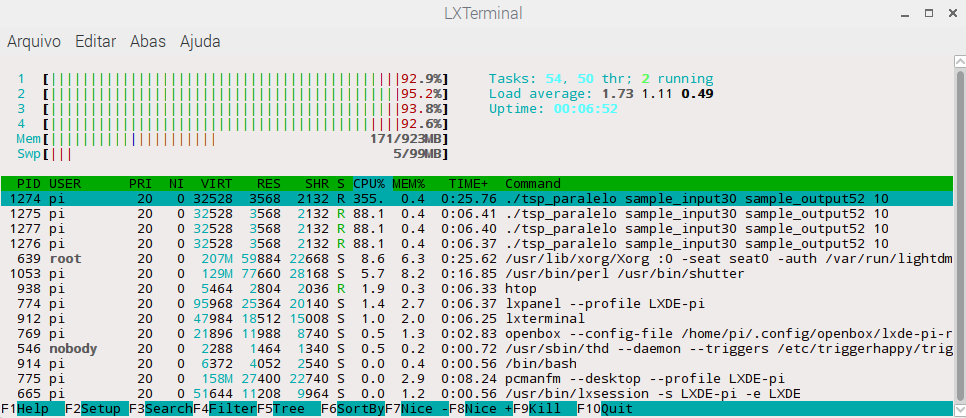
\includegraphics[width=.9\textwidth]{figuras/res_013}
	\caption[Raspberry Pi: AG paralelo]{Raspberry Pi: AG paralelo, em que é possível ver as \textit{threads} criadas durante a execução.}
	\label{figura:res_013}
\end{figure}

\begin{figure}[htb]  
	\centering
	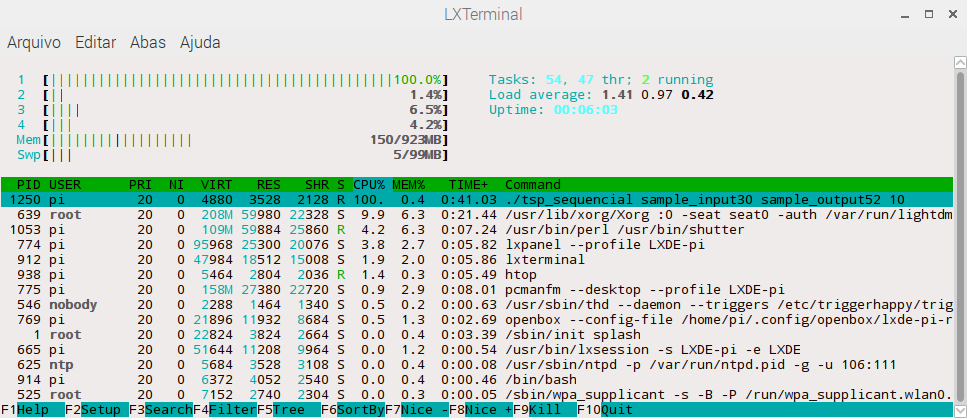
\includegraphics[width=.9\textwidth]{figuras/res_014}
	\caption[Raspberry Pi: AG sequencial]{Raspberry Pi: AG sequencial, em que é possível ver a única \textit{thread} criada durante a execução.}
	\label{figura:res_014}
\end{figure}

\begin{figure}[htb]  
	\centering
	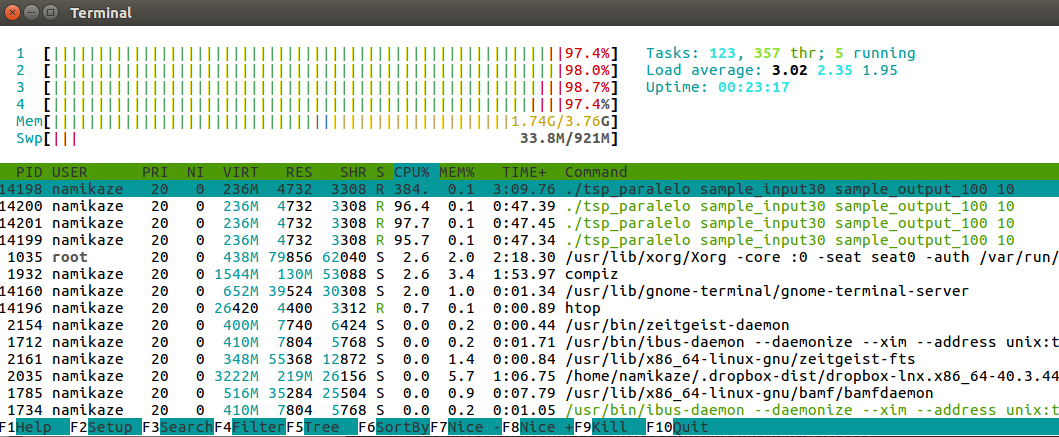
\includegraphics[width=.9\textwidth]{figuras/res_015}
	\caption[\textit{Notebook}:AG paralelo]{\textit{Notebook}:AG paralelo, em que é possível ver as \textit{threads} criadas durante a execução.}
	\label{figura:res_015}
\end{figure}

\begin{figure}[htb]  
	\centering
	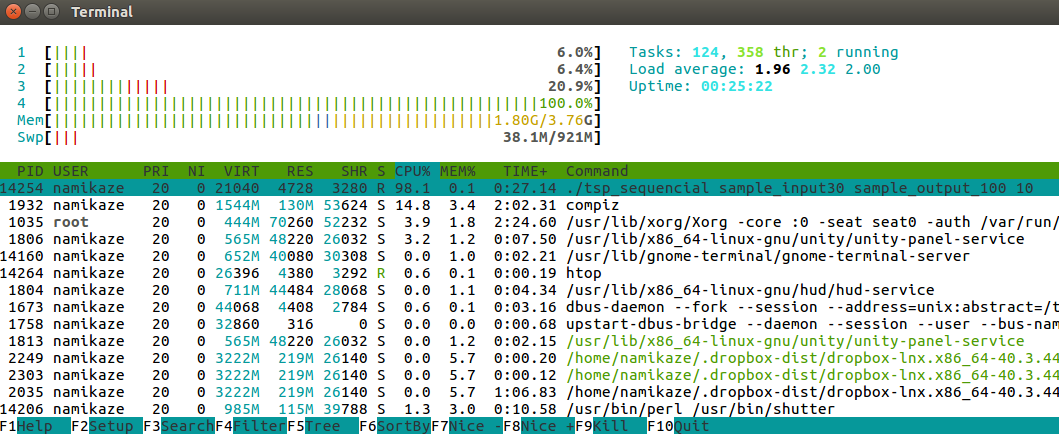
\includegraphics[width=.9\textwidth]{figuras/res_016}
	\caption[\textit{Notebook}: AG sequencia]{\textit{Notebook}: AG sequencial, em que é possível ver a única \textit{thread} criada durante a execução.}
	\label{figura:res_016}
\end{figure}


Após a realização do primeiro teste, que variava o tamanho da entrada, foi possível analisar o comportamento de cada arquitetura tanto no AG paralelo quanto no sequencial. A Figura \ref{figura:res_001} mostra o gráfico obtido do AG sequencial e a  Figura \ref{figura:res_002} mostra o gráfico obtido do AG paralelo executados no \textit{notebook}.

\begin{figure}[htb]  
	\centering
	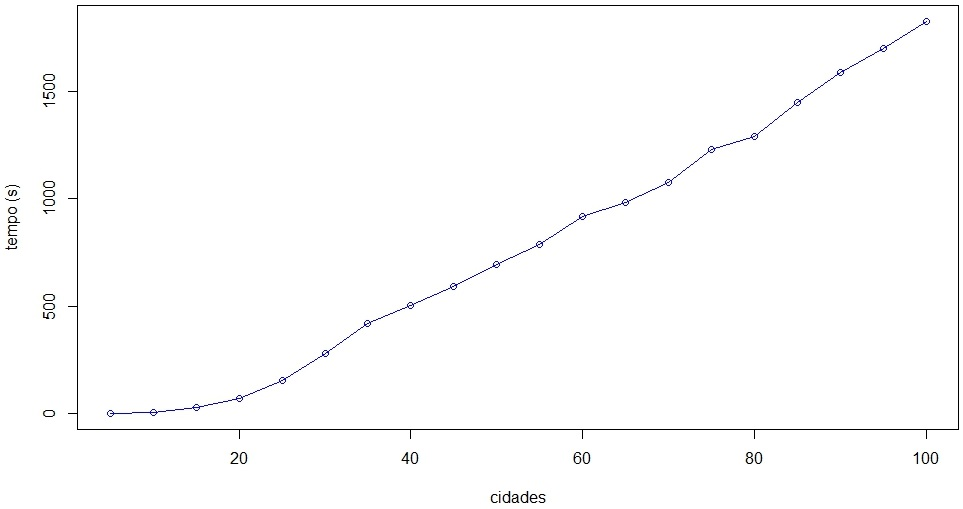
\includegraphics[width=.69\textwidth]{figuras/res_001_20nts}
	\caption[\textit{Notebook}: tempo sequencial]{\textit{Notebook}: Tempo em função da quantidade de cidades no algoritmo sequencial.}
	\label{figura:res_001}
\end{figure}

\begin{figure}[htb]  
	\centering
	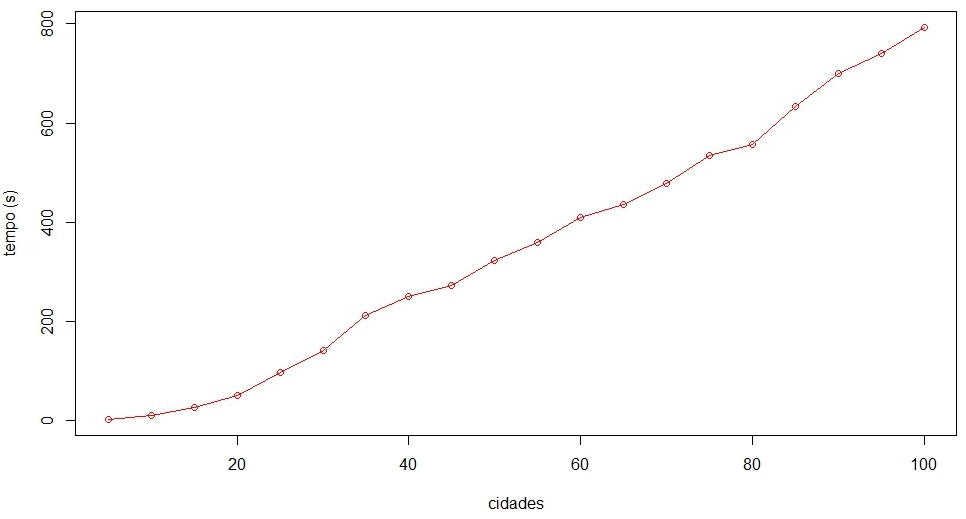
\includegraphics[width=.69\textwidth]{figuras/res_002_20ntp}
	\caption[\textit{Notebook}: tempo paralelo]{\textit{Notebook}: Tempo em função da quantidade de cidades no algoritmo paralelo.}
	\label{figura:res_002}
\end{figure}

As Figuras \ref{figura:res_003} e \ref{figura:res_004} mostram, respectivamente, os gráficos obtidos do AG sequencial e paralelo executados na placa Raspberry Pi.

\begin{figure}[htb]  
	\centering
	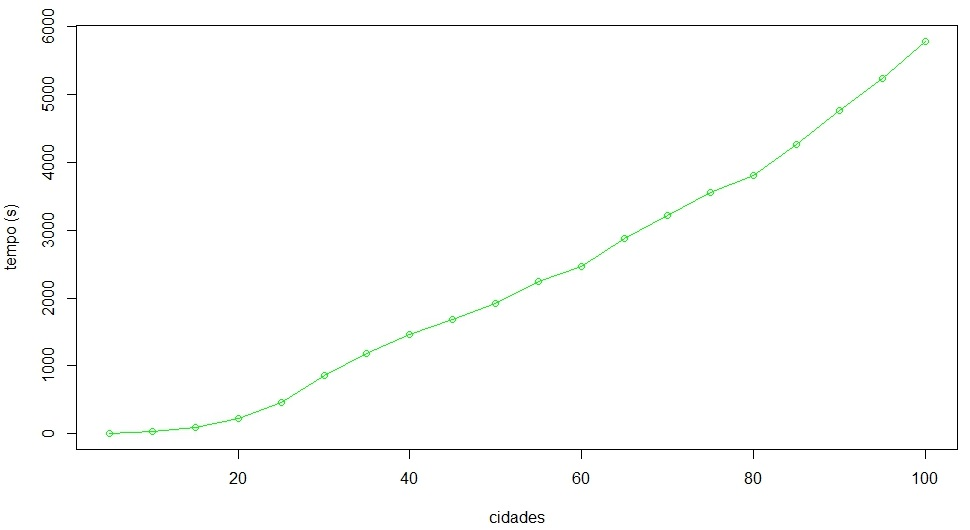
\includegraphics[width=.69\textwidth]{figuras/res_003_20rts}
	\caption[Raspberry Pi: tempo sequencial]{Raspberry Pi: Tempo em função da quantidade de cidades no algoritmo sequencial.}
	\label{figura:res_003}
\end{figure}

\begin{figure}[htb]  
	\centering
	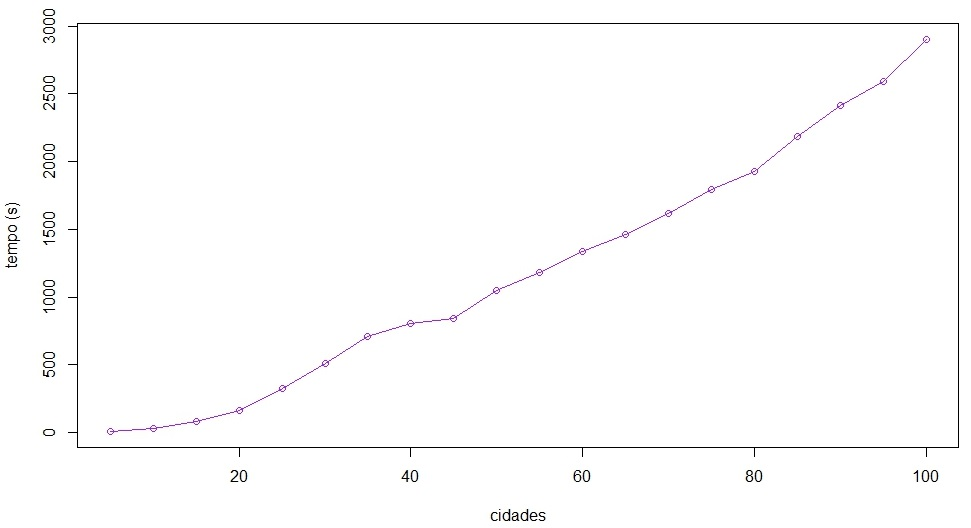
\includegraphics[width=.69\textwidth]{figuras/res_004_20rtp}
	\caption[Raspberry Pi: tempo paralelo]{Raspberry Pi: Tempo em função da quantidade de cidades no algoritmo paralelo.}
	\label{figura:res_004}
\end{figure} 

Observando-se as Figuras \ref{figura:res_001}, \ref{figura:res_002}, \ref{figura:res_003} e \ref{figura:res_004}, pode-se perceber que as arquiteturas apresentam comportamento semelhantes no AG tanto  sequencial quanto no paralelo. O que diferencia é a escala de tempo, já que em cada cenário apresentou faixas de tempo diferentes. É possível notar, também, que o aumento do tempo não apresentou forma exponencial, mas aproximadamente linear. Isso se deve ao uso de heurísticas (na implementação do AG) para resolução de problemas da classe NP-Difícil.

Com base nos tempos adiquiridos, foram calculados o $Sd$ e a $Ef$, que são mostrados na Tabela \ref{tabela:mostragem20}. É possível perceber que o $Sd$ do \textit{notebook} em relação a Raspberry Pi (no AG sequencial e no paralelo) é de aproximadamente 3,3 maior. Ao analisar o $Sd$ do $Tp$ em relação ao $Ts$ do \textit{notebook}, nota-se que o paralelo é quase duas vezes mais rápido que o sequencial. Já no $Sd$ do $Tp$ em relação ao $Ts$ da placa Raspberry Pi, o paralelo é aproximadamente 1,7 vezes mais rápido que o sequencial. As duas arquiteturas apresentaram valores bem próximos de $Ef$, sendo aproximadamente 50\% para o \textit{notebook} e 48\% para a Raspberry Pi.

%j
\begin{table}[htb] \centering
	\caption{Resultados - que incluem a média, mediana e desvio padrão - obtidos a parir do teste realizado com vinte repetições de execução, variando o tamanho das entradas, em cada um dos cenários propostos.} \label{tabela:mostragem20}
	\begin{tabular}{l|ccc}        \hline
		\textbf{Parâmetro analisado} & \textbf{Média} & \textbf{Mediana} & \textbf{Desvio Padrão} \\ \hline \hline		
		\textbf{\textit{Sd Ts} Raspberry/Notebook} 	& 3,2695	& 2,9558 & 1,0925	\\
		\textbf{\textit{Sd Tp} Raspberry/Notebook} 	& 3,3224	& 3,3456 & 0,1667	\\
		\textbf{\textit{Sd} Notebook \textit{Ts/Tp}}		 	& 1,9123	& 2,1792 & 0,5637	\\
		\textbf{\textit{Sd} Raspberry \textit{Ts/Tp}}		 	& 1,7350	& 1,8731 & 0,3314	\\
		\textbf{\textit{Ef} Notebook}			 	& 50,1549	& 54,4800 & 22,9936	\\
		\textbf{\textit{Ef} Raspberry}			 	& 47,9383	& 48,1387 & 21,9332	\\ \hline
	\end{tabular}
\end{table}

As Figuras \ref{figura:res_005} e \ref{figura:res_006} mostram, respectivamente, o comportamento da $Ef$ das arquiteturas conforme a quantidade de cidades no arquivo de entrada. Ao observá-las, fica evidente que a $Ef$ melhora com o aumento da carga de processamento. Isso se deve ao fato de que para pequenas cargas, o custo para divisão das tarefas (alocação e escalonamento de \textit{threads}, por exemplo) reduz a eficiência (aumenta o tempo da execução paralela) das arquiteturas.

\begin{figure}[htb]  
	\centering
	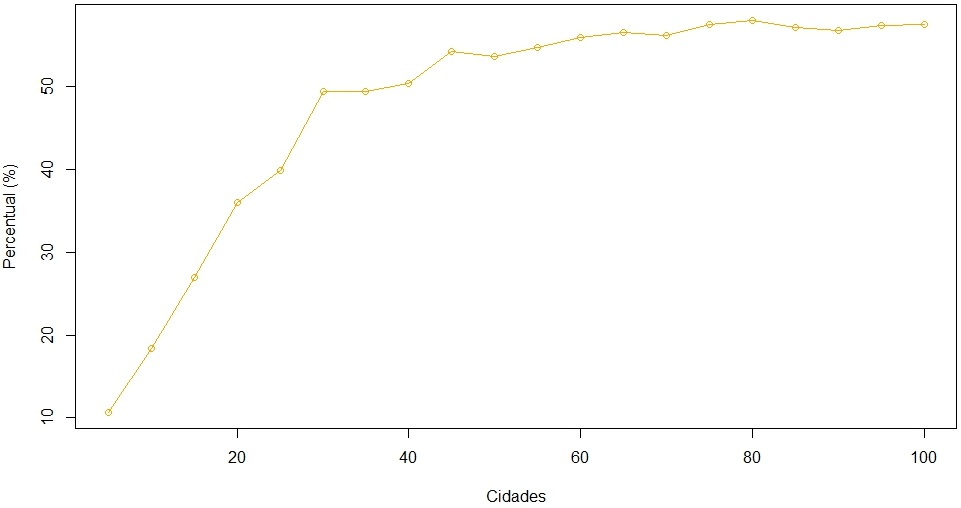
\includegraphics[width=.69\textwidth]{figuras/res_005_20efnt}
	\caption[\textit{Notebook}: eficiência]{\textit{Notebook}: Comportamento da eficiência em função do tamanho das entradas (quantidade de cidades).}
	\label{figura:res_005}
\end{figure} 

\begin{figure}[htb]  
	\centering
	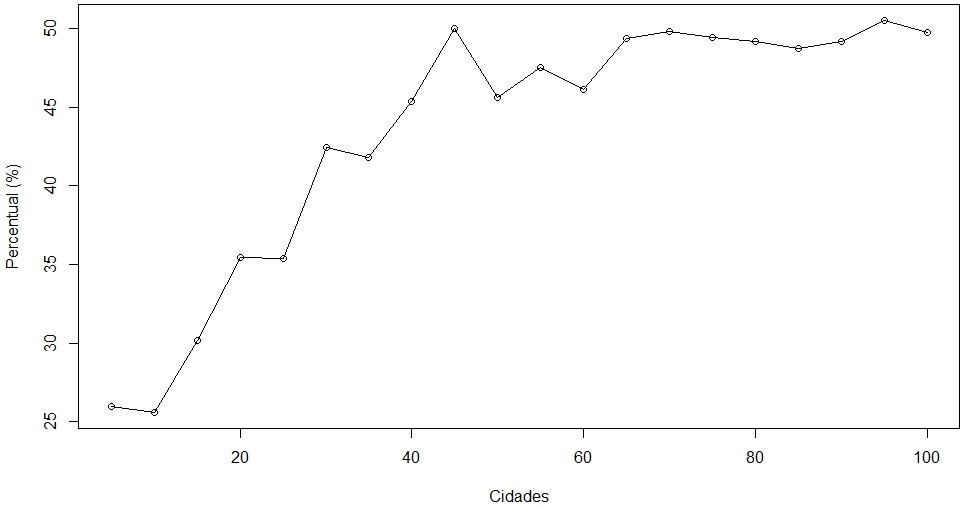
\includegraphics[width=.69\textwidth]{figuras/res_006_20efrp}
	\caption[Raspberry Pi: eficiância]{Raspberry Pi: Comportamente do eficiência em função do tamanho das entradas (quantidade de cidades).}
	\label{figura:res_006}
\end{figure} 

Ao analisar a Figura \ref{figura:res_007}, pode-se perceber a distribuição das medianas dos $Sd_s$ obtidos no primeiro teste, onde é possível notar alguns valores discrepantes (ou \textit{outliers}) no $Sd$ do \textit{notebook} em relação a Raspberry Pi, o que justifica o desvio padrão (Tabela \ref{tabela:mostragem20}) um pouco maior que os demais $Sd_s$ apresentados. Esses valores são resultados de execuções anormais se comparados com a maioria e, mesmo sendo \textit{outliers}, são normais e esperados em sistemas de propósito geral, visto que esses executam outras aplicações ao mesmo tempo, fazendo com que vários fatores interfiram no tempo total de execução.

\begin{figure}[htb]  
	\centering
	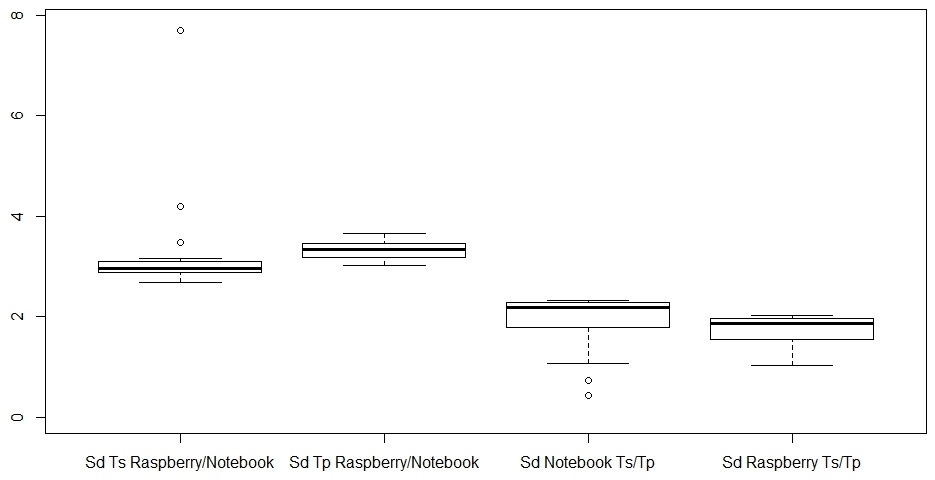
\includegraphics[width=.95\textwidth]{figuras/res_007_20sd}
	\caption[Comparação dos $Sd_s$ obtidos no primeiro teste]{Comparação dos $Sd_s$ obtidos no primeiro teste. O gráfico Boxplot mostra a comparação entre as medianas dos $Sd_s$ obtidos, além de suas variâncias.}
	\label{figura:res_007}
\end{figure} 

No segundo teste, foram repetidas 50 execuções do AG sequencial e paralelo nas duas arquiteturas, sem variar a quantidade de cidades, que foi fixada em 30. Dessa forma, foi possível analisar o comportamento das arquiteturas ao longo do tempo. As Figuras \ref{figura:res_008} e \ref{figura:res_009} apresentam os histogramas de $Ts_s$, $Tp_s$ e $Sd_s$ obtidos no segundo teste.

\begin{figure}[htb]  
	\centering
	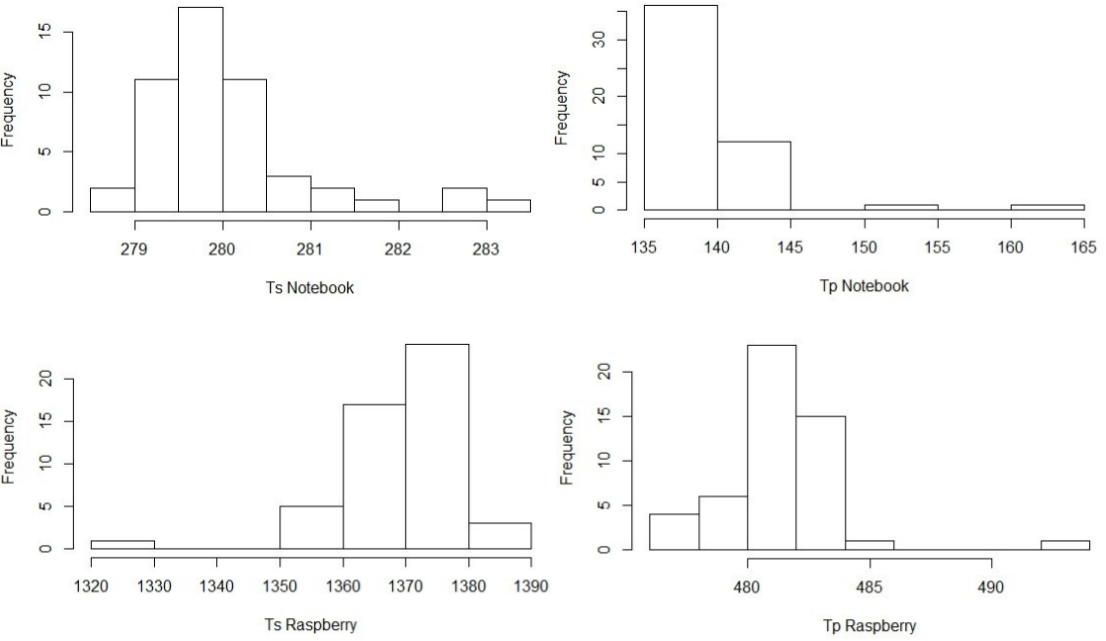
\includegraphics[width=.95\textwidth]{figuras/res_008_50tp}
	\caption[Histogramas dos tempos de execução obtidos]{Histogramas: Os gráficos mostram a frequência das ocorrências dos tempos de execução do AG, em todos os cenários, obtidos no segundo teste.}
	\label{figura:res_008}
\end{figure} 

\begin{figure}[htb]  
	\centering
	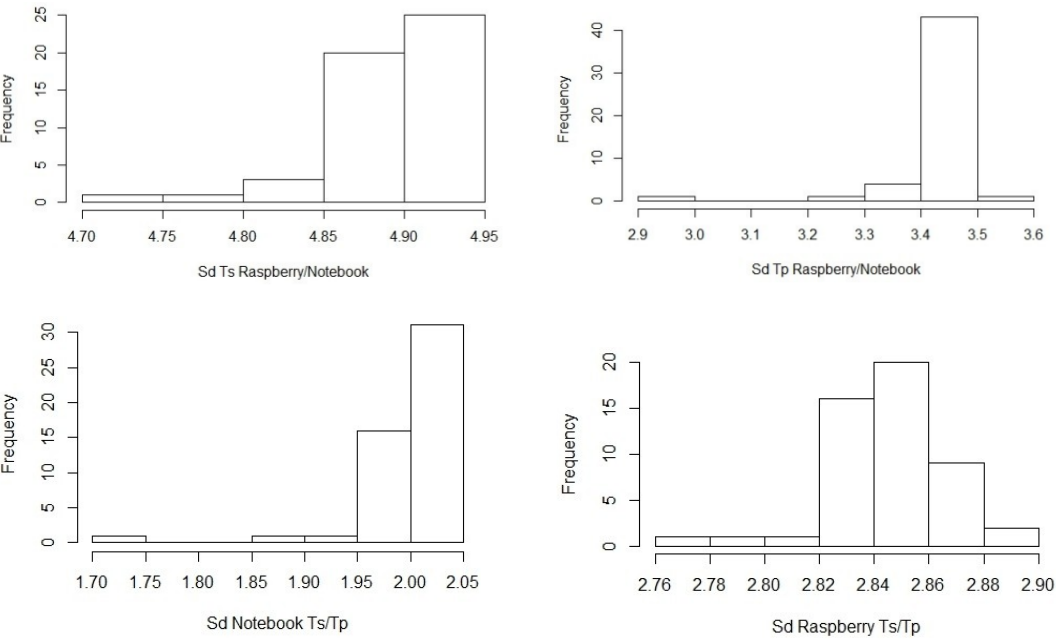
\includegraphics[width=.95\textwidth]{figuras/res_009_50sd}
	\caption[Histogramas dos $Sd_s$ obtidos]{Histogramas: Os gráficos mostram a frequência dos $Sd_s$ ocorridos nos diferentes cenários propostos, obtidos no segundo teste.}
	\label{figura:res_009}
\end{figure} 

Ao analisar a frequência dos tempos de execução, Figura \ref{figura:res_008}, pode-se observar que as arquiteturas apresentaram certa estabilidade nas execuções, visto que ouve pouca variação dos tempos nas faixas de maior frequência. A mesma situação ocorre na Figura \ref{figura:res_009} (frequências altas em faixas pequenas), com os valores de $Sd_s$. A execução sequencial na Raspberry Pi foi a que apresentou maior variabilidade nos tempos. Todos os cenários apresentam alguns valores discrepantes, porém os mesmos são esperados e considerados normais em arquiteturas de propósito geral. A Tabela \ref{tabela:mostragem50} mostra a média, mediana e desvio padrão dos tempos de execução sequenciais e paralelos, $Sd_s$ e $Ef$ das arquiteturas analisadas, que mostram resultados levemente diferentes aos obtidos no primeiro teste: o \textit{notebook} 4,8 vezes mais rápido que a Raspberry Pi no $Ts$ e 3,4 vezes mais rápido no tempo paralelo, o AG paralelo é 1,9 vezes mais rápido que o sequencial no \textit{notebook} e na Raspberry Pi é 2,8 vezes mais rápido.

%j
\begin{table}[htb] \centering
	\caption{Resultados - que incluem a média, mediana e desvio padrão - obtidos a parir do teste realizado com 50 repetições de execuções, com entrada de tamanho fixo, em cada um dos cenários propostos.} \label{tabela:mostragem50}
	\begin{tabular}{l|ccc}        \hline
		\textbf{Parâmetro analisado} & \textbf{Média} & \textbf{Mediana} & \textbf{Desvio Padrão} \\ \hline \hline
		\textbf{\textit{Ts} Notebook}			& 279,7962		  & 279,7430		 & 0,5213	\\
		\textbf{\textit{Ts} Raspberry}			& 1370,545		  & 1373,180		 & 7,0393	\\
		\textbf{\textit{Tp} Notebook}			& 139,5995		  & 139,5775		 & 0,3903	\\
		\textbf{\textit{Tp} Raspberry}			& 481,2862		  & 481,3365		 & 1,5111	\\
		\textbf{\textit{Sd Ts} Raspberry/Notebook} & 4,8897		  & 4,8995			 & 0,0381	\\
		\textbf{\textit{Sd Tp} Raspberry/Notebook} & 3,4266		  & 3,4439			 & 0,0785	\\
		\textbf{\textit{Sd} Notebook \textit{Ts/Tp}}		& 1,9936		  & 2,0032			 & 0,0456	\\
		\textbf{\textit{Sd} Raspberry \textit{Ts/Tp}}		& 2,8449		  & 2,8466			 & 0,0213	\\
		\textbf{\textit{Ef} Notebook}			& 49,8415		  & 50,081			 & 1,1407	\\
		\textbf{\textit{Ef} Raspberry}			& 71,1238		  & 71,165			 & 0,5339	\\ \hline
	\end{tabular}
\end{table}
%j 

As Figuras \ref{figura:res_011} e \ref{figura:res_012} mostram o comportamento, respectivamente, das $Ef_s$ do \textit{notebook} e da Raspberry Pi no decorrer da execuções. Com base nestas imagens e nos valores de $Ef$ apresentados na Tabela \ref{tabela:mostragem50}, nota-se que a Raspberry obteve uma eficiência melhor se comparada ao \textit{notebook}. Isso se deve principalmente as otimizações a nível de SO da placa, por ser um sistema mais limitado em relação ao \textit{notebook}, que permitiram um melhor aproveitamento dos núcleos.

\begin{figure}[htb]  
	\centering
	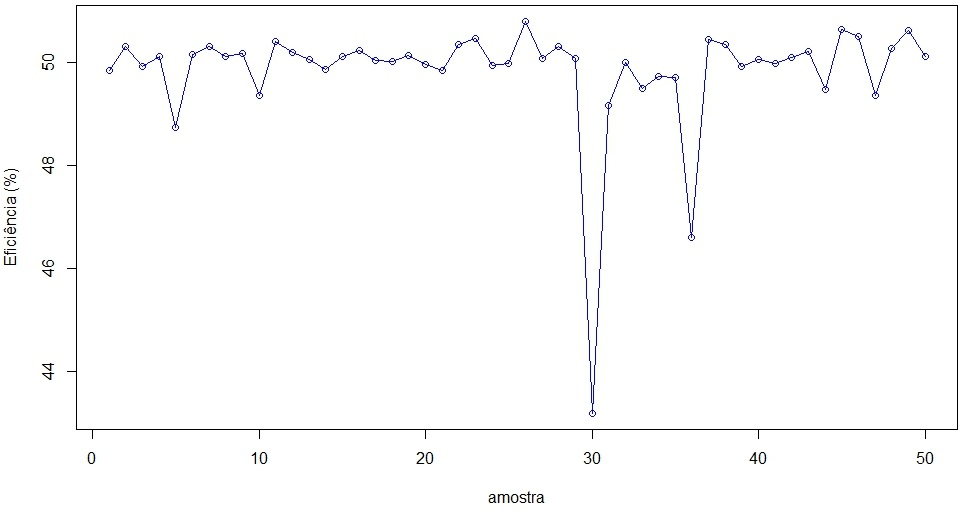
\includegraphics[width=\textwidth]{figuras/res_011_50efnt}
	\caption[\textit{Notebook}: eficiência]{\textit{Notebook}: Comportamento da $Ef$ do \textit{notebook} ao longo das execuções com entradas do mesmo tamanho.}
	\label{figura:res_011}
\end{figure}  

\begin{figure}[htb]  
	\centering
	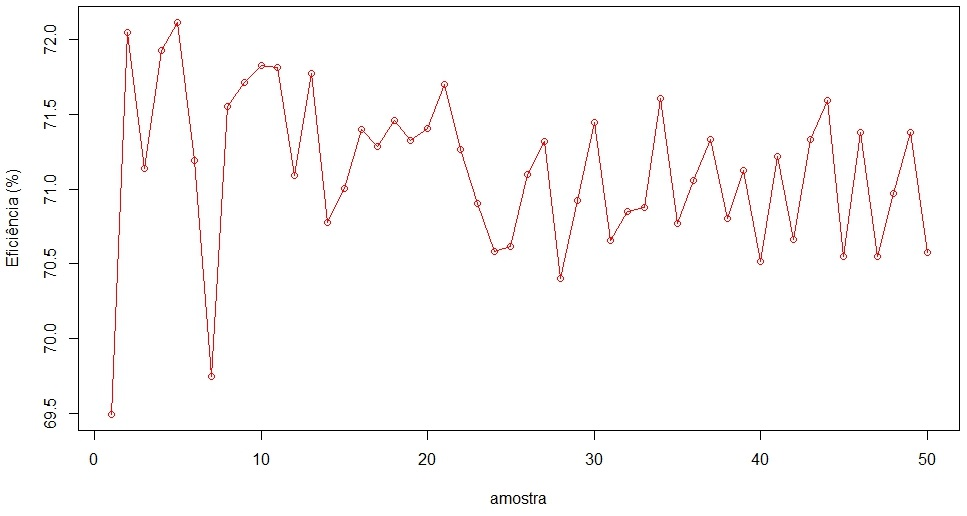
\includegraphics[width=\textwidth]{figuras/res_012_50efrp}
	\caption[Raspberry Pi: eficiência]{Raspberry Pi: Comportamento da $Ef$ da placa Raspberry Pi ao longo das execuções com entradas do mesmo tamanho.}
	\label{figura:res_012}
\end{figure}

\chapter{Conclusões}

Neste trabalho foi realizado um comparativo de desempenho entre um computador \textit{desktop} e uma Raspberry Pi. Para a realização dos testes, um AG para resolução do PCV foi utilizado de forma sequencial e paralela (uso da biblioteca OpenMP). Foram realizados dois testes, sendo que o primeiro era a execução do AG com entradas de tamanhos diferentes e o segundo execuções repetidas (total de 50) com tamanho de entrada fixo (30 cidades) em ambas as arquiteturas propostas. Com o tempo de execução obtido, foram aplicadas as métricas como $Sd$ e $Ef$, entre outras, para análise do desempenho e comportamento das arquiteturas.

Os resultados mostram um $Sd$ de 3 a 4,8 do \textit{notebook} em relação a Raspberry Pi no AG sequencial e um $Sd$ em torno de 3,3 do \textit{notebook} em relação a Raspberry Pi no AG paralelo. Estes resultados são esperados visto que a placa possui recursos mais limitados em relação ao \textit{notebook}, dos quais podemos destacar:

\begin{enumerate}
	\item Memória secundária: o armazenamento da Raspberry Pi é um cartão MicroSD (memória \textit{flash}) que é mais lenta se comparada a do \textit{notebook} (HD SATA).
	
	\item Memória primária: a memória da Raspberry Pi (DDR2 900 MHz) possui frequência menor que a do \textit{notebook} (DDR3 1,33GHz).
	
	\item Arquitetura x86 (híbrida de RISC e CISC) do \textit{notebook} possui instruções complexas já implementadas, enquanto que a arquitetura ARM (puramente RISC) não tem, o que aumenta a quantidade de instruções necessárias para executar determinadas tarfeas, se comparada com a x86.
\end{enumerate}

Por outro lado, a placa Raspberry Pi apresentou melhor eficiência na utilização de seus núcleos quando comparada com o \textit{notebook}. Isso se deve principalmente a otimização e robustez presentes da placa devido ao fato de ter seus recursos mais limitados, o que inclui um SO mais enchuto.

Por fim, pode-se concluir que a placa Raspberry Pi possui desempenho significativo que, aliado a outras vantagens (baixo custo, estabilidade, recursos como porta \textit{ethernet}, wi-fi, GPIO, entre outros), torna a placa uma alternativa barata e eficiente para aplicações de baixo custo e que não necessitam de tempo de resposta como fator crítico.

Pode-se destacar como principais limitações a falta de um ambiente de rede (\textit{cluster}) para testes com aplicações distribuídas, falta de testes com outros tipos de aplicações que exijam carga de processamento e análises utilizando softwares do tipo \textit{benchmark}. O consumo de energia e o desempenho com e sem um dissipador de calor para a Raspberry Pi também não foram analisados.

Como sugestão para trabalhos futuros:

\begin{enumerate}
	\item Testes com aplicações distribuídas, como por exemplo, utilizando \textit{cluster} homogêneo.
	
	\item Testes com aplicações distribuídas, como por exemplo, utilizando \textit{cluster} heterogêneo.
	
	\item Comparação com dispositivos similares a Raspberry Pi, por exemplo, a Orange Pi e a BeagleBone, entre outras.
	
	\item Testes com outras classes de algoritmos, por exemplo, para processamento gráfico, processamento de digital de imagens (PDI), mineração de dados em grandes volumes de informações, entre outras.
	
	\item Análise do consumo de energia, calor dissipado e a diferença de desempenho com e sem um dissipador de calor para a placa.
\end{enumerate}

% -----------------------------------------------------------------------------
% Elementos pós-textuais
% -----------------------------------------------------------------------------
\postextual

% -----------------------------------------------------------------------------
% Referências bibliográficas
% -----------------------------------------------------------------------------
\bibliography{referencias}

% -----------------------------------------------------------------------------
% Apêndices
% -----------------------------------------------------------------------------
%\apendices\partapendices

%\chapter{Documento Básico Usando a Classe {IF\TeX}}

%\begin{Verbatim}[frame=single, fontsize=\scriptsize]
\documentclass[english,brazil]{iftex} % Documento utilizando a classe iftex

\titulo{Título do trabalho}         % Título
\autor{Nome do Autor}               % Autor
\instituicao{Instituto Federal de Educação, Ciência e Tecnologia de Minas Gerais - Campus
Bambuí}                      % Instituição
\local{Bambuí - MG}                 % Local
\data{1}{junho}{2017}               % Data da defesa

\instituicao{Instituto Federal Minas Gerais} % Instituição
\unidade{Campus Bambuí}             % Unidade do IF
\tipotrabalho{monografia}           % monografia, dissertacao ou tese
\curso{Bacharel}{Engenharia de Computação}  % Título obtido e Curso

\areaconcentracao{Processamento de Textos}   % Área de concentração
\orientador{Nome do Orientador}              % Orientador
\coorientador[Coorientadora]{Nome da Coorientadora}     % Coorientadora
\coorientadorinstituicao{Instituição da Coorientadora}

% Membros da banca examinadora (além do orientador e coorientador)
\membrobanca{Fulando de Tal}{Instituição do Fulano de Tal}
\membrobanca{Ciclano de Tal}{Instituição do Ciclano de Tal}

\inserirfichacatalografica{ficha_catalografica} % Ficha catalográfica
\inserirfolhaaprovacao{}                        % Folha de aprovação

\inserirdedicatoria{
  Texto da dedicatória.
}

\inseriragradecimentos{
  Texto dos agradecimentos.
}

\inserirepigrafe{
  ``As invenções são, sobretudo, o resultado de um trabalho teimoso.''\\
  (Santos Dumont)
}

\resumo{
  Texto do resumo.
}
\palavraschave{Palavras. Chave;}

\abstract{
  Texto do abstract.
}
\keywords{English. Keywords.}

\inserirlistafiguras                     % Lista de Figuras
\inserirlistaquadros                     % Lista de Quadros
\inserirlistatabelas                     % Lista de Tabelas
\inserirlistaalgoritmos                  % Lista de Algoritmos
\inserirlistacodigos                     % Lista de Códigos
\inserirlistasiglas{\begin{itemize}[]
\item[ABNT] - Associação Brasileira de Normas Técnicas
\item[IFMG] - Instituto Federal de Educação, Ciência e Tecnologia de Minas Gerais
\item[SQL] - \textit{Structured Query Language}
\item[TCC] - Trabalho de conclusão de curso
\end{itemize}
}      % Lista de Siglas
\inserirlistasimbolos{\begin{itemize}[]
  \item $\mathbb{X}$ -- Variável X
  \item $\mathsf{I\!R}$ -- Conjunto dos números reais
\end{itemize}
}  % Lista de Símbolos

% Início do documento
\begin{document}

\maketitle

\chapter{Introdução}

Capítulo de Introdução

\chapter{Desenvolvimento}

Capítulo de Desenvolvimento

\chapter{Conclusão}

Capítulo de conclusão

\postextual

\bibliography{referencias}

\apendices\partapendices

\chapter{Título do Apêndice}

Conteúdo do apêndice

\anexos\partanexos

\chapter{Título do Anexo}

Conteúdo do anexo.

\end{document}
\end{Verbatim}


% -----------------------------------------------------------------------------
% Anexos
% -----------------------------------------------------------------------------
%\anexos\partanexos

%\chapter{Páginas Interessantes na Internet} \label{capitulo:paginas_interessantes}

%\begin{description}
 \item[\url{http://en.wikibooks.org/wiki/LaTeX}:] Livro em formato \textit{wiki} gratuito sobre {\LaTeX} (possui uma versão em português, mas a versão em inglês é a mais completa);
 \item[\url{http://tobi.oetiker.ch/lshort/lshort.pdf}:] Ótimo tutorial sobre {\LaTeX};
 \item[\url{abntex.codigolivre.org.br}:] Página do projeto \textit{abnTeX2} com informações sobre os pacotes e classes em {\LaTeX} para as normas da ABNT, nos quais a classe {IF\TeX} foi baseada.
\end{description}


\end{document}
